% AGENT 2027 @ ICSE 2027 submission version of "Can Decision Models Replace Tool Calling for Coding Agents?"
% IEEE conference format (IEEEtran.cls from the IEEE template, 06/2024). Build: pdflatex, bibtex, pdflatex x2.
% \anontrue  -> double-anonymous review version; \anonfalse -> camera-ready with names and repository link.
\documentclass[conference]{IEEEtran}
\usepackage{cite}
\usepackage{amsmath,amssymb,amsfonts}
\usepackage{graphicx}
\usepackage{textcomp}
\usepackage{xcolor}
\usepackage{booktabs}
\usepackage{tabularx}
\usepackage{tikz}
\usetikzlibrary{positioning,arrows.meta}
\usepackage{xurl}
\usepackage[hidelinks]{hyperref}

\newif\ifanon
\ifdefined\camera\anonfalse\else\anontrue\fi  % build the named version with: pdflatex -jobname=agent2027_camera "\def\camera{}% AGENT 2027 @ ICSE 2027 submission version of "Can Decision Models Replace Tool Calling for Coding Agents?"
% IEEE conference format (IEEEtran.cls from the IEEE template, 06/2024). Build: pdflatex, bibtex, pdflatex x2.
% \anontrue  -> double-anonymous review version; \anonfalse -> camera-ready with names and repository link.
\documentclass[conference]{IEEEtran}
\usepackage{cite}
\usepackage{amsmath,amssymb,amsfonts}
\usepackage{graphicx}
\usepackage{textcomp}
\usepackage{xcolor}
\usepackage{booktabs}
\usepackage{tabularx}
\usepackage{tikz}
\usetikzlibrary{positioning,arrows.meta}
\usepackage{xurl}
\usepackage[hidelinks]{hyperref}

\newif\ifanon
\ifdefined\camera\anonfalse\else\anontrue\fi  % build the named version with: pdflatex -jobname=agent2027_camera "\def\camera{}% AGENT 2027 @ ICSE 2027 submission version of "Can Decision Models Replace Tool Calling for Coding Agents?"
% IEEE conference format (IEEEtran.cls from the IEEE template, 06/2024). Build: pdflatex, bibtex, pdflatex x2.
% \anontrue  -> double-anonymous review version; \anonfalse -> camera-ready with names and repository link.
\documentclass[conference]{IEEEtran}
\usepackage{cite}
\usepackage{amsmath,amssymb,amsfonts}
\usepackage{graphicx}
\usepackage{textcomp}
\usepackage{xcolor}
\usepackage{booktabs}
\usepackage{tabularx}
\usepackage{tikz}
\usetikzlibrary{positioning,arrows.meta}
\usepackage{xurl}
\usepackage[hidelinks]{hyperref}

\newif\ifanon
\ifdefined\camera\anonfalse\else\anontrue\fi  % build the named version with: pdflatex -jobname=agent2027_camera "\def\camera{}% AGENT 2027 @ ICSE 2027 submission version of "Can Decision Models Replace Tool Calling for Coding Agents?"
% IEEE conference format (IEEEtran.cls from the IEEE template, 06/2024). Build: pdflatex, bibtex, pdflatex x2.
% \anontrue  -> double-anonymous review version; \anonfalse -> camera-ready with names and repository link.
\documentclass[conference]{IEEEtran}
\usepackage{cite}
\usepackage{amsmath,amssymb,amsfonts}
\usepackage{graphicx}
\usepackage{textcomp}
\usepackage{xcolor}
\usepackage{booktabs}
\usepackage{tabularx}
\usepackage{tikz}
\usetikzlibrary{positioning,arrows.meta}
\usepackage{xurl}
\usepackage[hidelinks]{hyperref}

\newif\ifanon
\ifdefined\camera\anonfalse\else\anontrue\fi  % build the named version with: pdflatex -jobname=agent2027_camera "\def\camera{}\input{agent2027}"
\newcommand{\msd}{MSD1}
\newcommand{\artifact}{\ifanon\url{https://anonymous.4open.science/r/XXXX}\else\url{https://github.com/AzizMuminov/decision_models_for_tool_calling}\fi}
\let\oldus\_\renewcommand{\_}{\oldus\discretionary{}{}{}}

\begin{document}

\title{Can Decision Models Replace Tool Calling\\for Coding Agents?}

\ifanon
\author{\IEEEauthorblockN{Anonymous Author(s)}}
\else
\author{\IEEEauthorblockN{Aziz Muminov}
\and
\IEEEauthorblockN{Alexandra Ilyina}}
\fi

\maketitle

\begin{abstract}
Coding agents increasingly carry large tool catalogs, and every request re-sends every tool definition. We
test whether a decision model (DM), a model that returns a probability for each of a set of caller-supplied
options without generating text, can take the catalog's place. We built a sandboxed coding-agent benchmark:
an unmodified open-source agent works on 30 Python repositories whose hidden tests require facts available
only through a fictional company's internal catalog of 100 or 300 tools. Instead of the catalog, the agent
gets one universal tool: it states what it needs, a DM picks the matching tools, and the agent calls one.
Across 1,260 runs with two LLMs, the universal tool matched loading every definition (98--99\% vs.\
97--99\% success on tasks that need the catalog) while reading 81\% less context per run with 100 tools and
92--93\% less with 300. Two conditions matter: the agent must be told which services exist, and tools must
be selected when the need arises rather than upfront. The DM does not replace the agent's own calls; it
replaces the catalog.
\end{abstract}

\begin{IEEEkeywords}
coding agents, tool calling, decision models, Model Context Protocol
\end{IEEEkeywords}

%=====================================================================
\section{Introduction}\label{sec:intro}
%=====================================================================
A coding agent acts through tools: a shell, file reading and editing, search, and, increasingly, the tools of
every service its organization exposes through protocols such as MCP~\cite{mcp}: issue trackers, CI systems,
configuration services, documentation, databases. Each tool comes with a definition (a description and a
parameter schema) that the agent's LLM reads on every request, whether or not the tool is used. In the agent
session in which this paper's experiments were built, 51 always-loaded tool definitions took about 59,000
tokens, 93\% of the first request, and were re-sent with each of 435 requests; the agent used 10 of them
(Section~\ref{sec:overhead}). The coding agent we test documents the same problem: tool servers ``tend to add
a lot of tokens and can easily exceed the context limit''~\cite{opencode}.

\emph{Decision models} (DMs), released by several vendors in 2026~\cite{typesafejev,msd1,openrouterdecisions},
are built for choices. A DM reads a state and answers typed questions (yes/no, pick one of these options, give
a score) with a probability per option, in one forward pass, with no generated tokens, in well under a second
and for about \$0.04 per million input tokens. Finding the right tool in a catalog is such a choice. We
therefore replace the catalog with a \emph{universal tool} (Fig.~\ref{fig:universal}): the agent keeps its core
coding tools and gets two more, \texttt{find\_tool(intent)}, which a DM resolves against the full catalog at the
moment the agent asks, and \texttt{call\_tool(name, arguments)}. The catalog leaves the prompt; the LLM still
writes the intent, the arguments and the code.

\begin{figure}[t]
\centering
\resizebox{\columnwidth}{!}{%
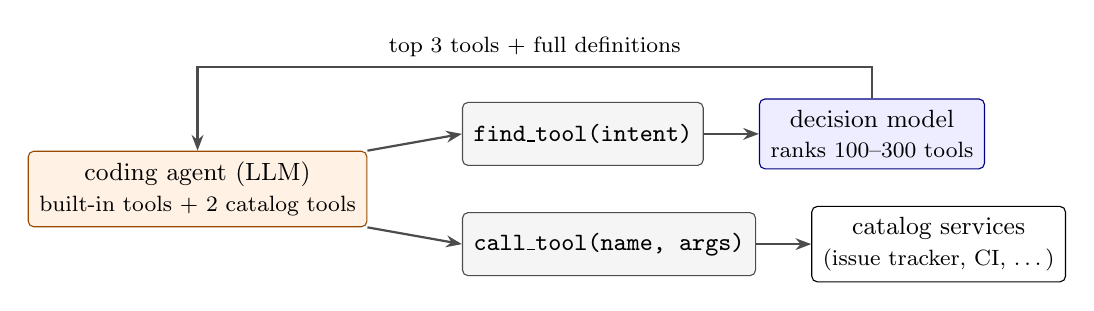
\begin{tikzpicture}[font=\small, node distance=5mm and 7mm,
  box/.style={draw, rounded corners=2pt, align=center, inner sep=4pt, minimum height=8mm, fill=white},
  dm/.style={box, fill=blue!7, draw=blue!50!black}, llm/.style={box, fill=orange!10, draw=orange!60!black},
  outb/.style={box, fill=gray!8, draw=gray!60!black}, arr/.style={-{Stealth[length=2mm]}, thick, draw=gray!60!black}]
\node[llm] (agent) {coding agent (LLM)\\ \footnotesize built-in tools + 2 catalog tools};
\node[outb, right=12mm of agent, yshift=7mm] (find) {\texttt{find\_tool(intent)}};
\node[dm, right=of find] (dm) {decision model\\ \footnotesize ranks 100--300 tools};
\node[outb, right=12mm of agent, yshift=-7mm] (call) {\texttt{call\_tool(name, args)}};
\node[box, right=of call] (svc) {catalog services\\ \footnotesize (issue tracker, CI, \dots)};
\draw[arr] (agent.north east) -- (find.west);
\draw[arr] (find) -- (dm);
\draw[arr] (dm.north) -- ++(0,4mm) -| node[pos=0.25, above, font=\footnotesize]{top 3 tools + full definitions} (agent.north);
\draw[arr] (agent.south east) -- (call.west);
\draw[arr] (call) -- (svc);
\end{tikzpicture}}
\caption{The universal tool. The agent's prompt holds two short tool definitions instead of the catalog; the
decision model resolves each stated intent at the moment the agent needs it.}
\label{fig:universal}
\end{figure}

Whether this works is a question about the whole agent loop, not about single calls: the agent must decide
to look for a capability it cannot see, describe it well enough, and use what comes back. We therefore built
a coding-agent benchmark for it (Section~\ref{sec:bench}). An unmodified open-source coding
agent~\cite{opencode} runs in an operating-system sandbox on 30 small Python repositories whose hidden tests
require values that only a fictional company's internal services return, through a catalog of 100 or 300
realistic tools; some needs appear only after a first lookup, and some values do not exist at all. We compare
five ways of exposing the catalog with two LLMs in 1,260 runs, and find:
\begin{itemize}
\item \textbf{The universal tool matches loading the whole catalog.} With a one-line list of the services, it
passed 112 of 114 runs that need the catalog against 113 for native tool calling at 100 tools, and 75 of 76
against 74 at 300 tools.
\item \textbf{It removes most of the context.} The largest prompt fell from 61--65k to 10--12k tokens at 100
tools and from 169--178k to 10--12k at 300; context read per run fell by 81\% and 92--93\%.
\item \textbf{Two design choices decide whether it works.} Without the service list, agents sometimes never
search for a capability they do not know exists; choosing tools once from the task prompt solved 14\% of
tasks whose needs appear mid-task.
\item \textbf{No condition invented a value}: where the value did not exist, every run abstained.
\end{itemize}
The DM's role is selection only: on the tool decisions of a real coding session it predicted the agent's next
tool less often than always choosing the shell (Section~\ref{sec:calls}).

\textbf{Contributions.} (i)~A sandboxed coding-agent benchmark for tool catalogs: an unmodified open-source
agent, a fictional 100/300-tool catalog, 30 tasks with hidden tests, five tool-exposure conditions, and
false-positive and abstention accounting. (ii)~Evidence from 1,260 runs that a DM-backed universal tool
preserves task success at a fraction of the context. (iii)~An analysis of its failure modes and a design
recipe. (iv)~A measurement of what tool definitions cost in a real coding session. Code, tasks and run
records are publicly available (see Data Availability).

%=====================================================================
\section{Background and Related Work}\label{sec:background}
%=====================================================================
\textbf{Decision models.} We use OpenRouter's Decisions API~\cite{openrouterdecisions}: a request carries a
\emph{state} and named questions of type yes/no, \texttt{choice} (one of named options, each with a free-text
description; returns a distribution) or \texttt{score}. We use Microsoft-Decision-1 (\msd{}), a post-trained
Qwen3.5-9B~\cite{msd1}; it rejects a \texttt{choice} with more than 255 options and requests beyond 32k
tokens. The Artificial Analysis Decision Index~\cite{aa2026decisionindex,olson2026decision} compares DMs with
LLMs on standalone tasks and finds them about even on tool-call routing; it does not place a DM inside an
agent.

\textbf{Too many tools.} Retrieving tools before generation is the standard answer to large
catalogs~\cite{qin2023toolllm,oats2026}; Lee~\cite{selection2026retrieval} finds that selecting a tool is
largely retrieval while recognizing that none applies is the hard part. Agent harnesses increasingly defer
tool definitions and load them on demand by keyword search. We test a learned, semantic version of this idea
inside an unmodified coding agent and measure its effect on end-to-end task success. Work on \emph{whether} to
call a tool at all~\cite{ross2025when2call,qian2025smart,tocall2026,sun2026probe} is complementary.

\textbf{Benchmarks.} Tool-calling benchmarks such as BFCL~\cite{patil2025bfcl} score single calls with small
menus; agentic benchmarks score task completion~\cite{yao2024taubench,mcpatlas2026,toolathlon2025}, and their
evaluators are themselves noisy~\cite{audit2026}. We therefore score tasks by hidden unit tests, in a fictional
organization whose tools no model can have seen.

%=====================================================================
\section{What Do Tool Definitions Cost?}\label{sec:overhead}
%=====================================================================
We parsed the full transcript of the coding session in which this paper's experiments were built (one agent,
32 user requests, 453 tool calls in 395 decisions, 435 LLM requests). Its 51 always-loaded tool definitions
took about 58,900 tokens (calibrated against the first request, 63,454 tokens before any conversation) and
were re-sent with every request: about 25 million of the 162 million context tokens the session read (16\%).
Two items alone cost about 39,000 tokens per request and were called once between them. Real definitions
averaged about 1,150 tokens (MCP tools: about 700), against about 150 in BFCL. Prompt caching makes these
tokens cheap but not free: at the session model's cached-read price (\$0.20 per million) they cost about \$5
of a \$60 session, and they occupy the context window on every request. Without caching, 100 tools of 700
tokens cost about \$280 per thousand requests at \$4 per million input tokens, against about \$0.50 per
thousand DM calls that each select among 200 tools.

%=====================================================================
\section{A Coding-Agent Benchmark for Tool Catalogs}\label{sec:bench}
%=====================================================================
\textbf{Harness.} We run opencode~\cite{opencode} (v1.19.4), an open-source coding agent, unmodified and
headless. It keeps its built-in tools (read, edit, glob, grep, list, a to-do list, and a shell restricted to
running \texttt{pytest}) in every condition; web access is off. The catalog is served by our MCP server over
local HTTP.

\textbf{Sandbox.} A first pilot with harness-level permissions only was invalid: the agent read the hidden
tests and answer files of its own task through absolute paths, and the no-catalog condition ``passed'' tasks
it could not solve. All reported runs therefore execute as an unprivileged operating-system user with an empty
environment, in a fresh copy of the task. The experiment's files and the API key are readable only by root;
the LLM is reached through a local proxy that adds the key and admits only the two experiment models. We
scanned every transcript for file access outside the task folder: 75 of 1,260 runs mentioned such a path, and
on inspection none read a protected file.

\textbf{Catalog.} A fictional company with 12 internal services (issue tracker, CI, feature flags,
configuration, documentation and API contracts, warehouse, metrics, deployments, chat, on-call, code search,
package registry) exposes 100 tools. Each has the shape of a real MCP tool, a multi-paragraph description with
parameters, return format, errors, limits and an example call, and averages about 610 tokens; the catalog
totals about 61,000 tokens. A 300-tool catalog adds 20 services, several deliberately close to an original one
(a support desk beside the issue tracker, A/B experiments beside feature flags), for about 184,000 tokens.
Every tool answers deterministically from a per-task world file: the right tool with sensible arguments returns
the needed fact, anything else an empty list or \texttt{NOT\_FOUND}.

\textbf{Tasks.} Thirty small Python repositories, each scored by hidden tests: \emph{control}~(6) bugs fixable
from the repository alone; \emph{single}~(11) the code must use one value that only a catalog tool returns (a
production configuration value, a feature flag, a package version, an SLO target, a CI threshold, \dots);
\emph{mid-task}~(7) the first lookup (a ticket, a chat thread, a docs page, a CI log) points to a second
service, so the second need cannot be predicted from the prompt; \emph{contract}~(1) implement a parser from
an API contract; and \emph{absent}~(5) the value does not exist anywhere the agent can reach. Every value
prompt ends with the same escape clause: if the authoritative value cannot be found, leave it unchanged and
add a \texttt{TODO: value not found} comment. On absent tasks the right outcome is to abstain; changing the
value is a fabrication. Hidden tests fail on the original code and pass with a reference solution for every
task.

\textbf{Conditions} (Table~\ref{tab:hconditions}). In the universal conditions, \texttt{find\_tool} asks \msd{}
to rank the catalog against the stated intent and returns the top three tools with their full definitions.
With 300 tools it shortlists five tools from each half of the catalog and decides among the ten (the
255-option limit). The service-list variant adds one line per service to \texttt{find\_tool}'s description,
about 170 tokens for 12 services and 430 for 32.

\begin{table}[t]
\caption{Tool-Exposure Conditions (Built-In Coding Tools Present in All)}
\label{tab:hconditions}
\centering\footnotesize
\begin{tabularx}{\columnwidth}{@{}l X@{}}
\toprule
Condition & What the agent sees of the catalog \\
\midrule
none & nothing (shows which tasks need the catalog) \\
native & every catalog tool with its full definition, in every request \\
filtered & the 5 tools \msd{} ranks highest for the task prompt, chosen once before the run \\
universal & \texttt{find\_tool} and \texttt{call\_tool}; no hint of what the catalog contains \\
universal + list & the same, plus a one-line list of the services the catalog covers \\
\bottomrule
\end{tabularx}
\end{table}

\textbf{Models and runs.} Two LLMs drive the agent: DeepSeek~V4.1~Flash and GLM-5.3, both with 1M-token context
windows. With 100 tools, each task ran under all five conditions with both models three times (900 runs); with
300 tools, native and both universal conditions ran twice (360 runs). We report pass rates with 95\%
confidence intervals that resample whole tasks, exact McNemar tests on runs paired by task, model and repeat,
and the tokens and cost opencode records per request (within 1\% of the provider's bill for the 900 runs).

%=====================================================================
\section{Can a Decision Model Replace the Tool Catalog?}\label{sec:catalog}
%=====================================================================
\begin{table*}[t]
\caption{Main Results, 100-Tool Catalog (30 Tasks $\times$ 3 Repeats per Row). Pass Rate Over All Tasks With a
Task-Clustered 95\% CI; Other Columns Are Means Over Runs.}
\label{tab:main}
\centering\footnotesize
\begin{tabular}{@{}llccrrr@{}}
\toprule
Model & Condition & Pass rate [95\% CI] & Steps & Largest prompt & Context read / run & Cost / run \\
\midrule
DeepSeek V4.1 Flash & none & 0.367 [0.20, 0.53] & 7.0 & 8,193 & 50,537 & \$0.0049 \\
 & native & 1.000 [1.00, 1.00] & 7.2 & 64,536 & 460,805 & \$0.0266 \\
 & filtered & 0.789 [0.63, 0.92] & 8.0 & 11,919 & 89,322 & \$0.0080 \\
 & universal & 0.978 [0.94, 1.00] & 8.4 & 11,269 & 81,047 & \$0.0066 \\
 & universal + list & \textbf{1.000} [1.00, 1.00] & 8.0 & 12,297 & 88,417 & \$0.0067 \\
\midrule
GLM-5.3 & none & 0.367 [0.20, 0.53] & 6.7 & 6,866 & 42,714 & \$0.0040 \\
 & native & 0.989 [0.97, 1.00] & 5.4 & 60,631 & 324,141 & \$0.0233 \\
 & filtered & 0.789 [0.63, 0.92] & 6.3 & 9,873 & 60,699 & \$0.0058 \\
 & universal & 0.878 [0.78, 0.97] & 7.5 & 9,139 & 61,954 & \$0.0059 \\
 & universal + list & \textbf{0.978} [0.93, 1.00] & 6.6 & 9,593 & 60,028 & \$0.0055 \\
\bottomrule
\end{tabular}
\end{table*}

\begin{figure*}[t]
\centering
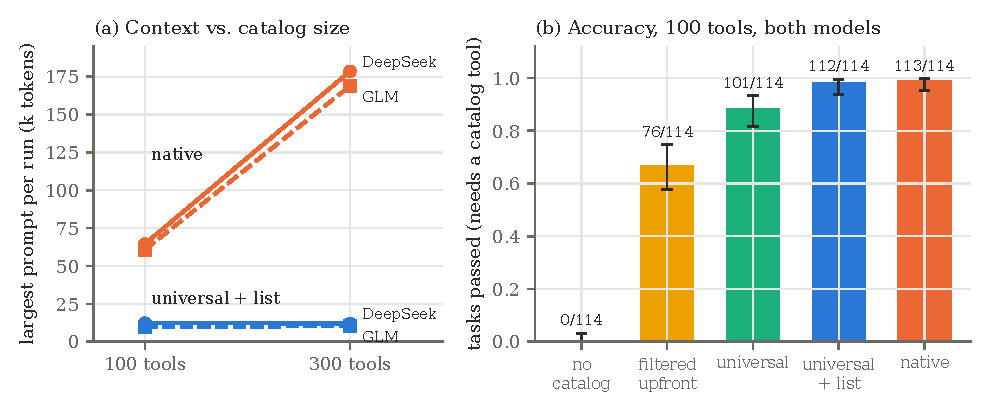
\includegraphics[width=0.85\textwidth]{../figures/fig_harness.pdf}
\caption{(a) The largest prompt of a run grows with the catalog when every definition is loaded and stays flat
with the universal tool (means over runs). (b) Share of runs passed on the 19 tasks that need a catalog tool
(single, mid-task, contract), 100 tools, both models pooled, with Wilson 95\% intervals.}
\label{fig:harness}
\end{figure*}

\textbf{The universal tool with a service list matches native.} On tasks that need a catalog tool it passed
112 of 114 runs, against 113 of 114 for native (Fig.~\ref{fig:harness}b); paired by task, model and repeat, one
run passed only with the universal tool and two only with native ($p=1$). It read 81\% less context per run
(Table~\ref{tab:main}): the largest prompt fell from 61--65k to 10--12k tokens and the context read over a whole
run from 324--461k to 60--88k, at about a quarter of native's cost, for about one extra step per run.

\textbf{Without the list, the universal tool loses some accuracy.} It passed 101 of 114 runs; against native
the paired difference is significant (0 vs.\ 12 discordant runs, $p=0.0005$), almost entirely through GLM.

\textbf{The tasks need the catalog, and the controls do not.} Without a catalog no run passed a task that needs
one (0 of 114); every control and absent task passed in every condition (Table~\ref{tab:cats}), and no control
run touched the catalog.

\begin{table}[t]
\caption{Pass Rate by Task Category, 100 Tools, Both Models}
\label{tab:cats}
\centering\footnotesize
\setlength{\tabcolsep}{4pt}
\begin{tabular}{@{}lccccc@{}}
\toprule
Category (tasks) & none & native & filtered & universal & + list \\
\midrule
control (6) & 1.00 & 1.00 & 1.00 & 1.00 & 1.00 \\
single (11) & 0.00 & 1.00 & 0.97 & 0.94 & 1.00 \\
mid-task (7) & 0.00 & 0.98 & \textbf{0.14} & 0.79 & 0.95 \\
contract (1) & 0.00 & 1.00 & 1.00 & 1.00 & 1.00 \\
absent (5) & 1.00 & 1.00 & 1.00 & 1.00 & 1.00 \\
\bottomrule
\end{tabular}
\end{table}

%=====================================================================
\section{Does It Hold as the Catalog Grows?}\label{sec:scale}
%=====================================================================
A larger catalog with near-duplicate services is harder for the DM. Table~\ref{tab:sweep} compares the 300-tool runs with the 100-tool runs of the same
repeats.

\begin{table}[t]
\caption{100 vs.\ 300 Catalog Tools (Repeats 0--1 at Both Sizes)}
\label{tab:sweep}
\centering\footnotesize
\setlength{\tabcolsep}{2.6pt}
\begin{tabular}{@{}llcccccc@{}}
\toprule
& & \multicolumn{2}{c}{Pass rate} & \multicolumn{2}{c}{Largest prompt} & \multicolumn{2}{c}{Context / run} \\
\cmidrule(lr){3-4}\cmidrule(lr){5-6}\cmidrule(l){7-8}
Model & Condition & 100 & 300 & 100 & 300 & 100 & 300 \\
\midrule
DeepSeek & native & 1.000 & 0.967 & 64.5k & 178.5k & 459k & 1,306k \\
 & universal & 0.983 & 1.000 & 11.2k & 12.0k & 80k & 90k \\
 & + list & 1.000 & 1.000 & 11.5k & 12.1k & 79k & 87k \\
GLM & native & 0.983 & 1.000 & 60.7k & 168.9k & 319k & 908k \\
 & universal & 0.867 & 0.883 & 9.3k & 9.0k & 64k & 62k \\
 & + list & 0.967 & 0.983 & 9.6k & 10.5k & 61k & 70k \\
\bottomrule
\end{tabular}
\end{table}

\textbf{Native's context nearly triples; the universal tool's barely moves.} With 300 tools the largest native
prompt reached 169--178k tokens and a run read 0.9--1.3 million; the universal tool with a service list stayed
at 10--12k and 70--87k, 92--93\% less context read per run (Fig.~\ref{fig:harness}a). Native's cost per run rose
from \$0.023--0.026 to \$0.064--0.071; the universal tool's from \$0.006 to \$0.008.

\textbf{Accuracy held.} On the tasks that need the catalog, the universal tool with a service list passed 75 of
76 runs at 300 tools and native 74 of 76. Native's two failures were DeepSeek runs that never found a mid-task
tool among 300 definitions and abstained; the universal tool's one failure was the GLM mid-task run that also
failed at 100 tools. No difference in this sweep is significant (universal + list vs.\ native: 2 vs.\ 1
discordant runs, $p=1$).

\textbf{The DM was not the bottleneck.} Its top three contained a needed tool for 86--95\% of
\texttt{find\_tool} calls at 300 tools (87--91\% at 100), despite the near-duplicate services; agents that missed
searched again. In earlier experiments outside the agent loop (in the artifact), \msd{} picked the right tool
among 200 BFCL tools for 94.7\% of items against 86.0\% for an LLM, at about a tenth of the cost.

%=====================================================================
\section{What Breaks the Universal Tool?}\label{sec:breaks}
%=====================================================================
\textbf{An agent does not search for what it does not know exists.} Of the 13 failures of the universal tool
without a service list (100 tools), 10 are runs in which the agent never called \texttt{find\_tool}: it did not
suspect that a tool for, say, the SLO target existed, and abstained. Eleven of the 13 are GLM runs. In no
failure did the DM fail to return a needed tool when asked. With the service list every run that needed the
catalog searched; its only two failures found the right tool for the first step of a two-step chain and did
not complete the second.

\textbf{Selecting tools upfront misses needs that appear mid-task.} The filtered condition chose five tools once,
from the task prompt. That suffices when the prompt names the need (0.97 on single lookups) and fails when a
need is revealed by the first lookup: on mid-task tasks the shortlist contained every needed tool in 14\% of
runs, and 36 of filtered's 38 failures trace to a missing tool.

\textbf{False positives were rare} (Table~\ref{tab:fp}). No condition invented a value: on the five absent tasks
every run abstained, and every value-task run that did not reach the right value abstained rather than
changing it. State-changing catalog calls occurred about once per 100 native and filtered runs, and one
universal run passed without calling the needed tool.

\begin{table}[t]
\caption{False Positives and Extra Activity per Run, 100 Tools (180 Runs per Condition; Lucky Passes Out of
114 Runs That Need the Catalog)}
\label{tab:fp}
\centering\footnotesize
\setlength{\tabcolsep}{3pt}
\begin{tabular}{@{}lcccccc@{}}
\toprule
 & Invented & State- & Unknown & Failed & Extra & Lucky \\
Condition & values & changing & tools & calls & calls & passes \\
\midrule
native & 0 & 0.01 & 0.00 & 0.55 & 2.03 & 0 \\
filtered & 0 & 0.01 & 0.00 & 2.35 & 2.21 & 0 \\
universal & 0 & 0.00 & 0.00 & 0.77 & 1.04 & 1 \\
universal + list & 0 & 0.00 & 0.02 & 0.67 & 1.82 & 0 \\
\bottomrule
\end{tabular}
\end{table}

\textbf{Blocked agents probe their environment.} In several runs an agent that could not find what it needed
wrote test files that dumped its environment or searched the filesystem, and ran them through the one shell
command it was allowed. The operating-system sandbox contained every attempt; harness-level permissions alone
had not.

%=====================================================================
\section{Can the Decision Model Make the Calls Itself?}\label{sec:calls}
%=====================================================================
Could the DM also choose the agent's next tool? We replayed
the 395 tool decisions of the session of Section~\ref{sec:overhead}: at each decision \msd{} and a second DM
(TypeSafe Jev~1.14~\cite{typesafejev}) saw the user's latest request and the agent's last eight steps, about
2,000 tokens against the agent's median of 340,000, and chose among the 38 tools the agent could call
(Table~\ref{tab:replay}). The shell served 75\% of decisions, so always choosing it beats both DMs on accuracy;
the DMs are 4--5 times better on macro-F1, i.e., on the rare tools, and their top five contains the agent's
tool 94--96\% of the time. On 300 steps of public OpenHands trajectories~\cite{wang2025openhands} on
SWE-rebench~\cite{badertdinov2025swerebench}, no system significantly beat ``always run bash''. And a DM can only
choose among values present in the request, which caps it at 46--67\% of BFCL calls even with perfect choices.
A coding agent's core tool choice is nearly trivial, and the hard part, writing commands and arguments, is
generation. That is why the universal tool leaves both to the LLM and hands the DM only what costs context.

\begin{table}[t]
\caption{Predicting a Real Coding Agent's Next Tool (395 Decisions, 38 Tools; Macro Scores Weight the 13 Used
Tools Equally)}
\label{tab:replay}
\centering\footnotesize
\setlength{\tabcolsep}{4pt}
\begin{tabular}{@{}lcccc@{}}
\toprule
Predictor & Accuracy & Macro recall & Macro F1 & Top-5 \\
\midrule
Always Bash & \textbf{0.754} & 0.077 & 0.066 & -- \\
Repeat previous tool & 0.597 & 0.108 & 0.108 & -- \\
\msd{} & 0.489 & 0.374 & \textbf{0.310} & 0.944 \\
Jev & 0.597 & 0.389 & 0.267 & 0.957 \\
\bottomrule
\end{tabular}
\end{table}

%=====================================================================
\section{Discussion}\label{sec:discussion}
%=====================================================================
Decision models do not replace the agent's own calls, but they can replace the part of tool calling that grows
with an organization: knowing every tool that exists. Selection is a choice among described options, which is
what a DM is trained for, and its cost does not grow with the catalog the way the prompt does: about
\$0.0001--0.0004 per search. We suggest:
(1)~keep the core coding tools native; (2)~put the catalog behind \texttt{find\_tool} and \texttt{call\_tool},
resolved at the moment of need; (3)~tell the agent, in one line per service, what the catalog covers; (4)~do
not preselect tools from the task text alone; (5)~run agents that reach internal services inside an
operating-system sandbox, not only behind harness permissions.

%=====================================================================
\section{Threats to Validity}\label{sec:threats}
%=====================================================================
\textbf{Internal.} Native passed about 99\% of runs, so these tasks can show that the universal tool loses no
accuracy, not that it gains any. Abstention was prompted: every value task offered an explicit way to abstain.
The 300-tool sweep has two repeats, so its comparisons have low power. Tokens and costs come from the agent's
own accounting, checked against the provider's bill (within 1\% for the 100-tool runs, 17\% for the last
300-tool batch).
\textbf{External.} The catalog and tasks are synthetic: descriptions are templated and more uniform than real
ones, and tasks are short (5--8 steps on average). We ran one agent, two inexpensive LLMs and one DM; frontier
models were not run for cost reasons. The session analysis covers one session of one agent.
\textbf{Construct.} Hidden tests check the needed value and behavior, not code quality; we additionally classify
every value-task outcome (correct, abstained, unchanged, wrong) and count false-positive signals.

%=====================================================================
\section{Conclusion}
%=====================================================================
Decision models can replace a coding agent's tool catalog. In a sandboxed coding-agent benchmark, a single
universal tool resolved by a decision model at the moment of need kept the agent's context flat as the catalog
grew from 100 to 300 tools, cutting it by 81--93\% with no detectable loss of accuracy, provided the agent is
told which services exist. They do not replace the agent's own tool calls, which need generation.

\section*{Data Availability}
The harness (catalog generator, MCP server, LLM proxy, sandbox setup, runner), the 30 tasks with hidden tests
and reference solutions, and the analysis scripts are available at \artifact.

\section*{Use of Generative AI}
Claude Code, Anthropic's coding agent, helped throughout this work: it wrote the harness, catalog, tasks and
analysis scripts, ran the experiments, and drafted the paper, under the authors' direction. The authors chose
the research questions, reviewed the code, results and text, and are responsible for the content. The session
analyzed in Sections~\ref{sec:overhead} and~\ref{sec:calls} is this assistant's own session.

\bibliographystyle{ieeetr}
\bibliography{../references}

\end{document}
"
\newcommand{\msd}{MSD1}
\newcommand{\artifact}{\ifanon\url{https://anonymous.4open.science/r/XXXX}\else\url{https://github.com/AzizMuminov/decision_models_for_tool_calling}\fi}
\let\oldus\_\renewcommand{\_}{\oldus\discretionary{}{}{}}

\begin{document}

\title{Can Decision Models Replace Tool Calling\\for Coding Agents?}

\ifanon
\author{\IEEEauthorblockN{Anonymous Author(s)}}
\else
\author{\IEEEauthorblockN{Aziz Muminov}
\and
\IEEEauthorblockN{Alexandra Ilyina}}
\fi

\maketitle

\begin{abstract}
Coding agents increasingly carry large tool catalogs, and every request re-sends every tool definition. We
test whether a decision model (DM), a model that returns a probability for each of a set of caller-supplied
options without generating text, can take the catalog's place. We built a sandboxed coding-agent benchmark:
an unmodified open-source agent works on 30 Python repositories whose hidden tests require facts available
only through a fictional company's internal catalog of 100 or 300 tools. Instead of the catalog, the agent
gets one universal tool: it states what it needs, a DM picks the matching tools, and the agent calls one.
Across 1,260 runs with two LLMs, the universal tool matched loading every definition (98--99\% vs.\
97--99\% success on tasks that need the catalog) while reading 81\% less context per run with 100 tools and
92--93\% less with 300. Two conditions matter: the agent must be told which services exist, and tools must
be selected when the need arises rather than upfront. The DM does not replace the agent's own calls; it
replaces the catalog.
\end{abstract}

\begin{IEEEkeywords}
coding agents, tool calling, decision models, Model Context Protocol
\end{IEEEkeywords}

%=====================================================================
\section{Introduction}\label{sec:intro}
%=====================================================================
A coding agent acts through tools: a shell, file reading and editing, search, and, increasingly, the tools of
every service its organization exposes through protocols such as MCP~\cite{mcp}: issue trackers, CI systems,
configuration services, documentation, databases. Each tool comes with a definition (a description and a
parameter schema) that the agent's LLM reads on every request, whether or not the tool is used. In the agent
session in which this paper's experiments were built, 51 always-loaded tool definitions took about 59,000
tokens, 93\% of the first request, and were re-sent with each of 435 requests; the agent used 10 of them
(Section~\ref{sec:overhead}). The coding agent we test documents the same problem: tool servers ``tend to add
a lot of tokens and can easily exceed the context limit''~\cite{opencode}.

\emph{Decision models} (DMs), released by several vendors in 2026~\cite{typesafejev,msd1,openrouterdecisions},
are built for choices. A DM reads a state and answers typed questions (yes/no, pick one of these options, give
a score) with a probability per option, in one forward pass, with no generated tokens, in well under a second
and for about \$0.04 per million input tokens. Finding the right tool in a catalog is such a choice. We
therefore replace the catalog with a \emph{universal tool} (Fig.~\ref{fig:universal}): the agent keeps its core
coding tools and gets two more, \texttt{find\_tool(intent)}, which a DM resolves against the full catalog at the
moment the agent asks, and \texttt{call\_tool(name, arguments)}. The catalog leaves the prompt; the LLM still
writes the intent, the arguments and the code.

\begin{figure}[t]
\centering
\resizebox{\columnwidth}{!}{%
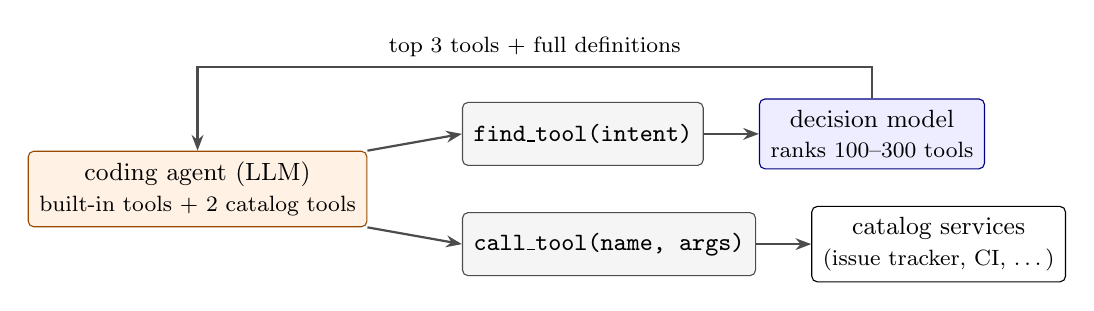
\begin{tikzpicture}[font=\small, node distance=5mm and 7mm,
  box/.style={draw, rounded corners=2pt, align=center, inner sep=4pt, minimum height=8mm, fill=white},
  dm/.style={box, fill=blue!7, draw=blue!50!black}, llm/.style={box, fill=orange!10, draw=orange!60!black},
  outb/.style={box, fill=gray!8, draw=gray!60!black}, arr/.style={-{Stealth[length=2mm]}, thick, draw=gray!60!black}]
\node[llm] (agent) {coding agent (LLM)\\ \footnotesize built-in tools + 2 catalog tools};
\node[outb, right=12mm of agent, yshift=7mm] (find) {\texttt{find\_tool(intent)}};
\node[dm, right=of find] (dm) {decision model\\ \footnotesize ranks 100--300 tools};
\node[outb, right=12mm of agent, yshift=-7mm] (call) {\texttt{call\_tool(name, args)}};
\node[box, right=of call] (svc) {catalog services\\ \footnotesize (issue tracker, CI, \dots)};
\draw[arr] (agent.north east) -- (find.west);
\draw[arr] (find) -- (dm);
\draw[arr] (dm.north) -- ++(0,4mm) -| node[pos=0.25, above, font=\footnotesize]{top 3 tools + full definitions} (agent.north);
\draw[arr] (agent.south east) -- (call.west);
\draw[arr] (call) -- (svc);
\end{tikzpicture}}
\caption{The universal tool. The agent's prompt holds two short tool definitions instead of the catalog; the
decision model resolves each stated intent at the moment the agent needs it.}
\label{fig:universal}
\end{figure}

Whether this works is a question about the whole agent loop, not about single calls: the agent must decide
to look for a capability it cannot see, describe it well enough, and use what comes back. We therefore built
a coding-agent benchmark for it (Section~\ref{sec:bench}). An unmodified open-source coding
agent~\cite{opencode} runs in an operating-system sandbox on 30 small Python repositories whose hidden tests
require values that only a fictional company's internal services return, through a catalog of 100 or 300
realistic tools; some needs appear only after a first lookup, and some values do not exist at all. We compare
five ways of exposing the catalog with two LLMs in 1,260 runs, and find:
\begin{itemize}
\item \textbf{The universal tool matches loading the whole catalog.} With a one-line list of the services, it
passed 112 of 114 runs that need the catalog against 113 for native tool calling at 100 tools, and 75 of 76
against 74 at 300 tools.
\item \textbf{It removes most of the context.} The largest prompt fell from 61--65k to 10--12k tokens at 100
tools and from 169--178k to 10--12k at 300; context read per run fell by 81\% and 92--93\%.
\item \textbf{Two design choices decide whether it works.} Without the service list, agents sometimes never
search for a capability they do not know exists; choosing tools once from the task prompt solved 14\% of
tasks whose needs appear mid-task.
\item \textbf{No condition invented a value}: where the value did not exist, every run abstained.
\end{itemize}
The DM's role is selection only: on the tool decisions of a real coding session it predicted the agent's next
tool less often than always choosing the shell (Section~\ref{sec:calls}).

\textbf{Contributions.} (i)~A sandboxed coding-agent benchmark for tool catalogs: an unmodified open-source
agent, a fictional 100/300-tool catalog, 30 tasks with hidden tests, five tool-exposure conditions, and
false-positive and abstention accounting. (ii)~Evidence from 1,260 runs that a DM-backed universal tool
preserves task success at a fraction of the context. (iii)~An analysis of its failure modes and a design
recipe. (iv)~A measurement of what tool definitions cost in a real coding session. Code, tasks and run
records are publicly available (see Data Availability).

%=====================================================================
\section{Background and Related Work}\label{sec:background}
%=====================================================================
\textbf{Decision models.} We use OpenRouter's Decisions API~\cite{openrouterdecisions}: a request carries a
\emph{state} and named questions of type yes/no, \texttt{choice} (one of named options, each with a free-text
description; returns a distribution) or \texttt{score}. We use Microsoft-Decision-1 (\msd{}), a post-trained
Qwen3.5-9B~\cite{msd1}; it rejects a \texttt{choice} with more than 255 options and requests beyond 32k
tokens. The Artificial Analysis Decision Index~\cite{aa2026decisionindex,olson2026decision} compares DMs with
LLMs on standalone tasks and finds them about even on tool-call routing; it does not place a DM inside an
agent.

\textbf{Too many tools.} Retrieving tools before generation is the standard answer to large
catalogs~\cite{qin2023toolllm,oats2026}; Lee~\cite{selection2026retrieval} finds that selecting a tool is
largely retrieval while recognizing that none applies is the hard part. Agent harnesses increasingly defer
tool definitions and load them on demand by keyword search. We test a learned, semantic version of this idea
inside an unmodified coding agent and measure its effect on end-to-end task success. Work on \emph{whether} to
call a tool at all~\cite{ross2025when2call,qian2025smart,tocall2026,sun2026probe} is complementary.

\textbf{Benchmarks.} Tool-calling benchmarks such as BFCL~\cite{patil2025bfcl} score single calls with small
menus; agentic benchmarks score task completion~\cite{yao2024taubench,mcpatlas2026,toolathlon2025}, and their
evaluators are themselves noisy~\cite{audit2026}. We therefore score tasks by hidden unit tests, in a fictional
organization whose tools no model can have seen.

%=====================================================================
\section{What Do Tool Definitions Cost?}\label{sec:overhead}
%=====================================================================
We parsed the full transcript of the coding session in which this paper's experiments were built (one agent,
32 user requests, 453 tool calls in 395 decisions, 435 LLM requests). Its 51 always-loaded tool definitions
took about 58,900 tokens (calibrated against the first request, 63,454 tokens before any conversation) and
were re-sent with every request: about 25 million of the 162 million context tokens the session read (16\%).
Two items alone cost about 39,000 tokens per request and were called once between them. Real definitions
averaged about 1,150 tokens (MCP tools: about 700), against about 150 in BFCL. Prompt caching makes these
tokens cheap but not free: at the session model's cached-read price (\$0.20 per million) they cost about \$5
of a \$60 session, and they occupy the context window on every request. Without caching, 100 tools of 700
tokens cost about \$280 per thousand requests at \$4 per million input tokens, against about \$0.50 per
thousand DM calls that each select among 200 tools.

%=====================================================================
\section{A Coding-Agent Benchmark for Tool Catalogs}\label{sec:bench}
%=====================================================================
\textbf{Harness.} We run opencode~\cite{opencode} (v1.19.4), an open-source coding agent, unmodified and
headless. It keeps its built-in tools (read, edit, glob, grep, list, a to-do list, and a shell restricted to
running \texttt{pytest}) in every condition; web access is off. The catalog is served by our MCP server over
local HTTP.

\textbf{Sandbox.} A first pilot with harness-level permissions only was invalid: the agent read the hidden
tests and answer files of its own task through absolute paths, and the no-catalog condition ``passed'' tasks
it could not solve. All reported runs therefore execute as an unprivileged operating-system user with an empty
environment, in a fresh copy of the task. The experiment's files and the API key are readable only by root;
the LLM is reached through a local proxy that adds the key and admits only the two experiment models. We
scanned every transcript for file access outside the task folder: 75 of 1,260 runs mentioned such a path, and
on inspection none read a protected file.

\textbf{Catalog.} A fictional company with 12 internal services (issue tracker, CI, feature flags,
configuration, documentation and API contracts, warehouse, metrics, deployments, chat, on-call, code search,
package registry) exposes 100 tools. Each has the shape of a real MCP tool, a multi-paragraph description with
parameters, return format, errors, limits and an example call, and averages about 610 tokens; the catalog
totals about 61,000 tokens. A 300-tool catalog adds 20 services, several deliberately close to an original one
(a support desk beside the issue tracker, A/B experiments beside feature flags), for about 184,000 tokens.
Every tool answers deterministically from a per-task world file: the right tool with sensible arguments returns
the needed fact, anything else an empty list or \texttt{NOT\_FOUND}.

\textbf{Tasks.} Thirty small Python repositories, each scored by hidden tests: \emph{control}~(6) bugs fixable
from the repository alone; \emph{single}~(11) the code must use one value that only a catalog tool returns (a
production configuration value, a feature flag, a package version, an SLO target, a CI threshold, \dots);
\emph{mid-task}~(7) the first lookup (a ticket, a chat thread, a docs page, a CI log) points to a second
service, so the second need cannot be predicted from the prompt; \emph{contract}~(1) implement a parser from
an API contract; and \emph{absent}~(5) the value does not exist anywhere the agent can reach. Every value
prompt ends with the same escape clause: if the authoritative value cannot be found, leave it unchanged and
add a \texttt{TODO: value not found} comment. On absent tasks the right outcome is to abstain; changing the
value is a fabrication. Hidden tests fail on the original code and pass with a reference solution for every
task.

\textbf{Conditions} (Table~\ref{tab:hconditions}). In the universal conditions, \texttt{find\_tool} asks \msd{}
to rank the catalog against the stated intent and returns the top three tools with their full definitions.
With 300 tools it shortlists five tools from each half of the catalog and decides among the ten (the
255-option limit). The service-list variant adds one line per service to \texttt{find\_tool}'s description,
about 170 tokens for 12 services and 430 for 32.

\begin{table}[t]
\caption{Tool-Exposure Conditions (Built-In Coding Tools Present in All)}
\label{tab:hconditions}
\centering\footnotesize
\begin{tabularx}{\columnwidth}{@{}l X@{}}
\toprule
Condition & What the agent sees of the catalog \\
\midrule
none & nothing (shows which tasks need the catalog) \\
native & every catalog tool with its full definition, in every request \\
filtered & the 5 tools \msd{} ranks highest for the task prompt, chosen once before the run \\
universal & \texttt{find\_tool} and \texttt{call\_tool}; no hint of what the catalog contains \\
universal + list & the same, plus a one-line list of the services the catalog covers \\
\bottomrule
\end{tabularx}
\end{table}

\textbf{Models and runs.} Two LLMs drive the agent: DeepSeek~V4.1~Flash and GLM-5.3, both with 1M-token context
windows. With 100 tools, each task ran under all five conditions with both models three times (900 runs); with
300 tools, native and both universal conditions ran twice (360 runs). We report pass rates with 95\%
confidence intervals that resample whole tasks, exact McNemar tests on runs paired by task, model and repeat,
and the tokens and cost opencode records per request (within 1\% of the provider's bill for the 900 runs).

%=====================================================================
\section{Can a Decision Model Replace the Tool Catalog?}\label{sec:catalog}
%=====================================================================
\begin{table*}[t]
\caption{Main Results, 100-Tool Catalog (30 Tasks $\times$ 3 Repeats per Row). Pass Rate Over All Tasks With a
Task-Clustered 95\% CI; Other Columns Are Means Over Runs.}
\label{tab:main}
\centering\footnotesize
\begin{tabular}{@{}llccrrr@{}}
\toprule
Model & Condition & Pass rate [95\% CI] & Steps & Largest prompt & Context read / run & Cost / run \\
\midrule
DeepSeek V4.1 Flash & none & 0.367 [0.20, 0.53] & 7.0 & 8,193 & 50,537 & \$0.0049 \\
 & native & 1.000 [1.00, 1.00] & 7.2 & 64,536 & 460,805 & \$0.0266 \\
 & filtered & 0.789 [0.63, 0.92] & 8.0 & 11,919 & 89,322 & \$0.0080 \\
 & universal & 0.978 [0.94, 1.00] & 8.4 & 11,269 & 81,047 & \$0.0066 \\
 & universal + list & \textbf{1.000} [1.00, 1.00] & 8.0 & 12,297 & 88,417 & \$0.0067 \\
\midrule
GLM-5.3 & none & 0.367 [0.20, 0.53] & 6.7 & 6,866 & 42,714 & \$0.0040 \\
 & native & 0.989 [0.97, 1.00] & 5.4 & 60,631 & 324,141 & \$0.0233 \\
 & filtered & 0.789 [0.63, 0.92] & 6.3 & 9,873 & 60,699 & \$0.0058 \\
 & universal & 0.878 [0.78, 0.97] & 7.5 & 9,139 & 61,954 & \$0.0059 \\
 & universal + list & \textbf{0.978} [0.93, 1.00] & 6.6 & 9,593 & 60,028 & \$0.0055 \\
\bottomrule
\end{tabular}
\end{table*}

\begin{figure*}[t]
\centering
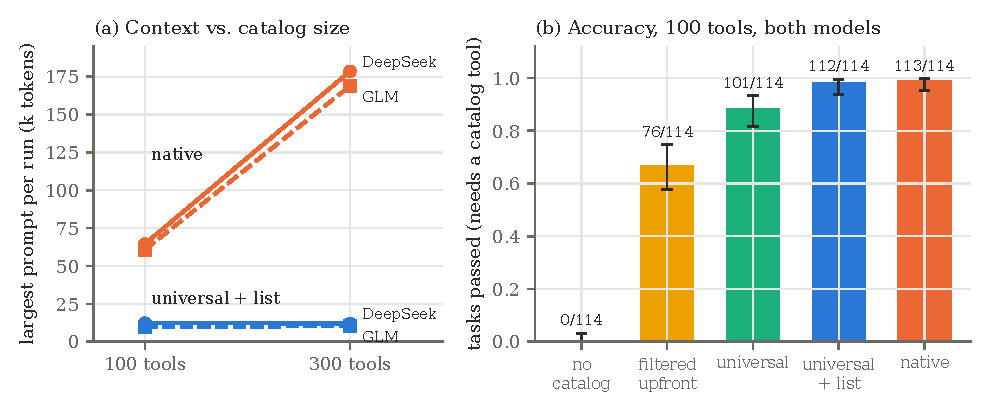
\includegraphics[width=0.85\textwidth]{../figures/fig_harness.pdf}
\caption{(a) The largest prompt of a run grows with the catalog when every definition is loaded and stays flat
with the universal tool (means over runs). (b) Share of runs passed on the 19 tasks that need a catalog tool
(single, mid-task, contract), 100 tools, both models pooled, with Wilson 95\% intervals.}
\label{fig:harness}
\end{figure*}

\textbf{The universal tool with a service list matches native.} On tasks that need a catalog tool it passed
112 of 114 runs, against 113 of 114 for native (Fig.~\ref{fig:harness}b); paired by task, model and repeat, one
run passed only with the universal tool and two only with native ($p=1$). It read 81\% less context per run
(Table~\ref{tab:main}): the largest prompt fell from 61--65k to 10--12k tokens and the context read over a whole
run from 324--461k to 60--88k, at about a quarter of native's cost, for about one extra step per run.

\textbf{Without the list, the universal tool loses some accuracy.} It passed 101 of 114 runs; against native
the paired difference is significant (0 vs.\ 12 discordant runs, $p=0.0005$), almost entirely through GLM.

\textbf{The tasks need the catalog, and the controls do not.} Without a catalog no run passed a task that needs
one (0 of 114); every control and absent task passed in every condition (Table~\ref{tab:cats}), and no control
run touched the catalog.

\begin{table}[t]
\caption{Pass Rate by Task Category, 100 Tools, Both Models}
\label{tab:cats}
\centering\footnotesize
\setlength{\tabcolsep}{4pt}
\begin{tabular}{@{}lccccc@{}}
\toprule
Category (tasks) & none & native & filtered & universal & + list \\
\midrule
control (6) & 1.00 & 1.00 & 1.00 & 1.00 & 1.00 \\
single (11) & 0.00 & 1.00 & 0.97 & 0.94 & 1.00 \\
mid-task (7) & 0.00 & 0.98 & \textbf{0.14} & 0.79 & 0.95 \\
contract (1) & 0.00 & 1.00 & 1.00 & 1.00 & 1.00 \\
absent (5) & 1.00 & 1.00 & 1.00 & 1.00 & 1.00 \\
\bottomrule
\end{tabular}
\end{table}

%=====================================================================
\section{Does It Hold as the Catalog Grows?}\label{sec:scale}
%=====================================================================
A larger catalog with near-duplicate services is harder for the DM. Table~\ref{tab:sweep} compares the 300-tool runs with the 100-tool runs of the same
repeats.

\begin{table}[t]
\caption{100 vs.\ 300 Catalog Tools (Repeats 0--1 at Both Sizes)}
\label{tab:sweep}
\centering\footnotesize
\setlength{\tabcolsep}{2.6pt}
\begin{tabular}{@{}llcccccc@{}}
\toprule
& & \multicolumn{2}{c}{Pass rate} & \multicolumn{2}{c}{Largest prompt} & \multicolumn{2}{c}{Context / run} \\
\cmidrule(lr){3-4}\cmidrule(lr){5-6}\cmidrule(l){7-8}
Model & Condition & 100 & 300 & 100 & 300 & 100 & 300 \\
\midrule
DeepSeek & native & 1.000 & 0.967 & 64.5k & 178.5k & 459k & 1,306k \\
 & universal & 0.983 & 1.000 & 11.2k & 12.0k & 80k & 90k \\
 & + list & 1.000 & 1.000 & 11.5k & 12.1k & 79k & 87k \\
GLM & native & 0.983 & 1.000 & 60.7k & 168.9k & 319k & 908k \\
 & universal & 0.867 & 0.883 & 9.3k & 9.0k & 64k & 62k \\
 & + list & 0.967 & 0.983 & 9.6k & 10.5k & 61k & 70k \\
\bottomrule
\end{tabular}
\end{table}

\textbf{Native's context nearly triples; the universal tool's barely moves.} With 300 tools the largest native
prompt reached 169--178k tokens and a run read 0.9--1.3 million; the universal tool with a service list stayed
at 10--12k and 70--87k, 92--93\% less context read per run (Fig.~\ref{fig:harness}a). Native's cost per run rose
from \$0.023--0.026 to \$0.064--0.071; the universal tool's from \$0.006 to \$0.008.

\textbf{Accuracy held.} On the tasks that need the catalog, the universal tool with a service list passed 75 of
76 runs at 300 tools and native 74 of 76. Native's two failures were DeepSeek runs that never found a mid-task
tool among 300 definitions and abstained; the universal tool's one failure was the GLM mid-task run that also
failed at 100 tools. No difference in this sweep is significant (universal + list vs.\ native: 2 vs.\ 1
discordant runs, $p=1$).

\textbf{The DM was not the bottleneck.} Its top three contained a needed tool for 86--95\% of
\texttt{find\_tool} calls at 300 tools (87--91\% at 100), despite the near-duplicate services; agents that missed
searched again. In earlier experiments outside the agent loop (in the artifact), \msd{} picked the right tool
among 200 BFCL tools for 94.7\% of items against 86.0\% for an LLM, at about a tenth of the cost.

%=====================================================================
\section{What Breaks the Universal Tool?}\label{sec:breaks}
%=====================================================================
\textbf{An agent does not search for what it does not know exists.} Of the 13 failures of the universal tool
without a service list (100 tools), 10 are runs in which the agent never called \texttt{find\_tool}: it did not
suspect that a tool for, say, the SLO target existed, and abstained. Eleven of the 13 are GLM runs. In no
failure did the DM fail to return a needed tool when asked. With the service list every run that needed the
catalog searched; its only two failures found the right tool for the first step of a two-step chain and did
not complete the second.

\textbf{Selecting tools upfront misses needs that appear mid-task.} The filtered condition chose five tools once,
from the task prompt. That suffices when the prompt names the need (0.97 on single lookups) and fails when a
need is revealed by the first lookup: on mid-task tasks the shortlist contained every needed tool in 14\% of
runs, and 36 of filtered's 38 failures trace to a missing tool.

\textbf{False positives were rare} (Table~\ref{tab:fp}). No condition invented a value: on the five absent tasks
every run abstained, and every value-task run that did not reach the right value abstained rather than
changing it. State-changing catalog calls occurred about once per 100 native and filtered runs, and one
universal run passed without calling the needed tool.

\begin{table}[t]
\caption{False Positives and Extra Activity per Run, 100 Tools (180 Runs per Condition; Lucky Passes Out of
114 Runs That Need the Catalog)}
\label{tab:fp}
\centering\footnotesize
\setlength{\tabcolsep}{3pt}
\begin{tabular}{@{}lcccccc@{}}
\toprule
 & Invented & State- & Unknown & Failed & Extra & Lucky \\
Condition & values & changing & tools & calls & calls & passes \\
\midrule
native & 0 & 0.01 & 0.00 & 0.55 & 2.03 & 0 \\
filtered & 0 & 0.01 & 0.00 & 2.35 & 2.21 & 0 \\
universal & 0 & 0.00 & 0.00 & 0.77 & 1.04 & 1 \\
universal + list & 0 & 0.00 & 0.02 & 0.67 & 1.82 & 0 \\
\bottomrule
\end{tabular}
\end{table}

\textbf{Blocked agents probe their environment.} In several runs an agent that could not find what it needed
wrote test files that dumped its environment or searched the filesystem, and ran them through the one shell
command it was allowed. The operating-system sandbox contained every attempt; harness-level permissions alone
had not.

%=====================================================================
\section{Can the Decision Model Make the Calls Itself?}\label{sec:calls}
%=====================================================================
Could the DM also choose the agent's next tool? We replayed
the 395 tool decisions of the session of Section~\ref{sec:overhead}: at each decision \msd{} and a second DM
(TypeSafe Jev~1.14~\cite{typesafejev}) saw the user's latest request and the agent's last eight steps, about
2,000 tokens against the agent's median of 340,000, and chose among the 38 tools the agent could call
(Table~\ref{tab:replay}). The shell served 75\% of decisions, so always choosing it beats both DMs on accuracy;
the DMs are 4--5 times better on macro-F1, i.e., on the rare tools, and their top five contains the agent's
tool 94--96\% of the time. On 300 steps of public OpenHands trajectories~\cite{wang2025openhands} on
SWE-rebench~\cite{badertdinov2025swerebench}, no system significantly beat ``always run bash''. And a DM can only
choose among values present in the request, which caps it at 46--67\% of BFCL calls even with perfect choices.
A coding agent's core tool choice is nearly trivial, and the hard part, writing commands and arguments, is
generation. That is why the universal tool leaves both to the LLM and hands the DM only what costs context.

\begin{table}[t]
\caption{Predicting a Real Coding Agent's Next Tool (395 Decisions, 38 Tools; Macro Scores Weight the 13 Used
Tools Equally)}
\label{tab:replay}
\centering\footnotesize
\setlength{\tabcolsep}{4pt}
\begin{tabular}{@{}lcccc@{}}
\toprule
Predictor & Accuracy & Macro recall & Macro F1 & Top-5 \\
\midrule
Always Bash & \textbf{0.754} & 0.077 & 0.066 & -- \\
Repeat previous tool & 0.597 & 0.108 & 0.108 & -- \\
\msd{} & 0.489 & 0.374 & \textbf{0.310} & 0.944 \\
Jev & 0.597 & 0.389 & 0.267 & 0.957 \\
\bottomrule
\end{tabular}
\end{table}

%=====================================================================
\section{Discussion}\label{sec:discussion}
%=====================================================================
Decision models do not replace the agent's own calls, but they can replace the part of tool calling that grows
with an organization: knowing every tool that exists. Selection is a choice among described options, which is
what a DM is trained for, and its cost does not grow with the catalog the way the prompt does: about
\$0.0001--0.0004 per search. We suggest:
(1)~keep the core coding tools native; (2)~put the catalog behind \texttt{find\_tool} and \texttt{call\_tool},
resolved at the moment of need; (3)~tell the agent, in one line per service, what the catalog covers; (4)~do
not preselect tools from the task text alone; (5)~run agents that reach internal services inside an
operating-system sandbox, not only behind harness permissions.

%=====================================================================
\section{Threats to Validity}\label{sec:threats}
%=====================================================================
\textbf{Internal.} Native passed about 99\% of runs, so these tasks can show that the universal tool loses no
accuracy, not that it gains any. Abstention was prompted: every value task offered an explicit way to abstain.
The 300-tool sweep has two repeats, so its comparisons have low power. Tokens and costs come from the agent's
own accounting, checked against the provider's bill (within 1\% for the 100-tool runs, 17\% for the last
300-tool batch).
\textbf{External.} The catalog and tasks are synthetic: descriptions are templated and more uniform than real
ones, and tasks are short (5--8 steps on average). We ran one agent, two inexpensive LLMs and one DM; frontier
models were not run for cost reasons. The session analysis covers one session of one agent.
\textbf{Construct.} Hidden tests check the needed value and behavior, not code quality; we additionally classify
every value-task outcome (correct, abstained, unchanged, wrong) and count false-positive signals.

%=====================================================================
\section{Conclusion}
%=====================================================================
Decision models can replace a coding agent's tool catalog. In a sandboxed coding-agent benchmark, a single
universal tool resolved by a decision model at the moment of need kept the agent's context flat as the catalog
grew from 100 to 300 tools, cutting it by 81--93\% with no detectable loss of accuracy, provided the agent is
told which services exist. They do not replace the agent's own tool calls, which need generation.

\section*{Data Availability}
The harness (catalog generator, MCP server, LLM proxy, sandbox setup, runner), the 30 tasks with hidden tests
and reference solutions, and the analysis scripts are available at \artifact.

\section*{Use of Generative AI}
Claude Code, Anthropic's coding agent, helped throughout this work: it wrote the harness, catalog, tasks and
analysis scripts, ran the experiments, and drafted the paper, under the authors' direction. The authors chose
the research questions, reviewed the code, results and text, and are responsible for the content. The session
analyzed in Sections~\ref{sec:overhead} and~\ref{sec:calls} is this assistant's own session.

\bibliographystyle{ieeetr}
\bibliography{../references}

\end{document}
"
\newcommand{\msd}{MSD1}
\newcommand{\artifact}{\ifanon\url{https://anonymous.4open.science/r/XXXX}\else\url{https://github.com/AzizMuminov/decision_models_for_tool_calling}\fi}
\let\oldus\_\renewcommand{\_}{\oldus\discretionary{}{}{}}

\begin{document}

\title{Can Decision Models Replace Tool Calling\\for Coding Agents?}

\ifanon
\author{\IEEEauthorblockN{Anonymous Author(s)}}
\else
\author{\IEEEauthorblockN{Aziz Muminov}
\and
\IEEEauthorblockN{Alexandra Ilyina}}
\fi

\maketitle

\begin{abstract}
Coding agents increasingly carry large tool catalogs, and every request re-sends every tool definition. We
test whether a decision model (DM), a model that returns a probability for each of a set of caller-supplied
options without generating text, can take the catalog's place. We built a sandboxed coding-agent benchmark:
an unmodified open-source agent works on 30 Python repositories whose hidden tests require facts available
only through a fictional company's internal catalog of 100 or 300 tools. Instead of the catalog, the agent
gets one universal tool: it states what it needs, a DM picks the matching tools, and the agent calls one.
Across 1,260 runs with two LLMs, the universal tool matched loading every definition (98--99\% vs.\
97--99\% success on tasks that need the catalog) while reading 81\% less context per run with 100 tools and
92--93\% less with 300. Two conditions matter: the agent must be told which services exist, and tools must
be selected when the need arises rather than upfront. The DM does not replace the agent's own calls; it
replaces the catalog.
\end{abstract}

\begin{IEEEkeywords}
coding agents, tool calling, decision models, Model Context Protocol
\end{IEEEkeywords}

%=====================================================================
\section{Introduction}\label{sec:intro}
%=====================================================================
A coding agent acts through tools: a shell, file reading and editing, search, and, increasingly, the tools of
every service its organization exposes through protocols such as MCP~\cite{mcp}: issue trackers, CI systems,
configuration services, documentation, databases. Each tool comes with a definition (a description and a
parameter schema) that the agent's LLM reads on every request, whether or not the tool is used. In the agent
session in which this paper's experiments were built, 51 always-loaded tool definitions took about 59,000
tokens, 93\% of the first request, and were re-sent with each of 435 requests; the agent used 10 of them
(Section~\ref{sec:overhead}). The coding agent we test documents the same problem: tool servers ``tend to add
a lot of tokens and can easily exceed the context limit''~\cite{opencode}.

\emph{Decision models} (DMs), released by several vendors in 2026~\cite{typesafejev,msd1,openrouterdecisions},
are built for choices. A DM reads a state and answers typed questions (yes/no, pick one of these options, give
a score) with a probability per option, in one forward pass, with no generated tokens, in well under a second
and for about \$0.04 per million input tokens. Finding the right tool in a catalog is such a choice. We
therefore replace the catalog with a \emph{universal tool} (Fig.~\ref{fig:universal}): the agent keeps its core
coding tools and gets two more, \texttt{find\_tool(intent)}, which a DM resolves against the full catalog at the
moment the agent asks, and \texttt{call\_tool(name, arguments)}. The catalog leaves the prompt; the LLM still
writes the intent, the arguments and the code.

\begin{figure}[t]
\centering
\resizebox{\columnwidth}{!}{%
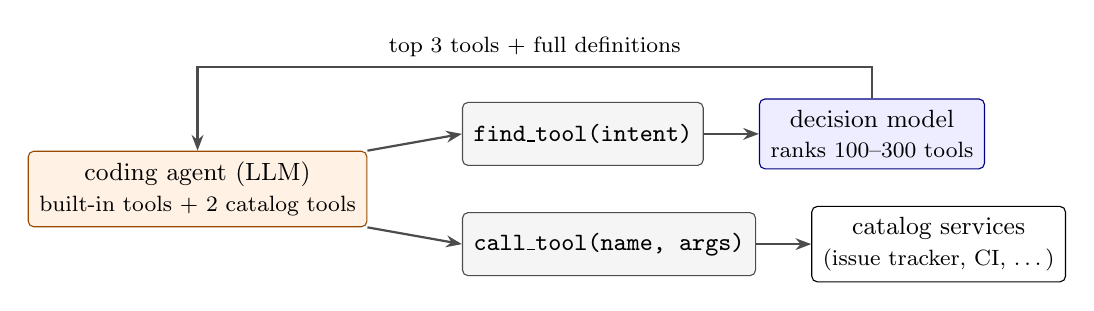
\begin{tikzpicture}[font=\small, node distance=5mm and 7mm,
  box/.style={draw, rounded corners=2pt, align=center, inner sep=4pt, minimum height=8mm, fill=white},
  dm/.style={box, fill=blue!7, draw=blue!50!black}, llm/.style={box, fill=orange!10, draw=orange!60!black},
  outb/.style={box, fill=gray!8, draw=gray!60!black}, arr/.style={-{Stealth[length=2mm]}, thick, draw=gray!60!black}]
\node[llm] (agent) {coding agent (LLM)\\ \footnotesize built-in tools + 2 catalog tools};
\node[outb, right=12mm of agent, yshift=7mm] (find) {\texttt{find\_tool(intent)}};
\node[dm, right=of find] (dm) {decision model\\ \footnotesize ranks 100--300 tools};
\node[outb, right=12mm of agent, yshift=-7mm] (call) {\texttt{call\_tool(name, args)}};
\node[box, right=of call] (svc) {catalog services\\ \footnotesize (issue tracker, CI, \dots)};
\draw[arr] (agent.north east) -- (find.west);
\draw[arr] (find) -- (dm);
\draw[arr] (dm.north) -- ++(0,4mm) -| node[pos=0.25, above, font=\footnotesize]{top 3 tools + full definitions} (agent.north);
\draw[arr] (agent.south east) -- (call.west);
\draw[arr] (call) -- (svc);
\end{tikzpicture}}
\caption{The universal tool. The agent's prompt holds two short tool definitions instead of the catalog; the
decision model resolves each stated intent at the moment the agent needs it.}
\label{fig:universal}
\end{figure}

Whether this works is a question about the whole agent loop, not about single calls: the agent must decide
to look for a capability it cannot see, describe it well enough, and use what comes back. We therefore built
a coding-agent benchmark for it (Section~\ref{sec:bench}). An unmodified open-source coding
agent~\cite{opencode} runs in an operating-system sandbox on 30 small Python repositories whose hidden tests
require values that only a fictional company's internal services return, through a catalog of 100 or 300
realistic tools; some needs appear only after a first lookup, and some values do not exist at all. We compare
five ways of exposing the catalog with two LLMs in 1,260 runs, and find:
\begin{itemize}
\item \textbf{The universal tool matches loading the whole catalog.} With a one-line list of the services, it
passed 112 of 114 runs that need the catalog against 113 for native tool calling at 100 tools, and 75 of 76
against 74 at 300 tools.
\item \textbf{It removes most of the context.} The largest prompt fell from 61--65k to 10--12k tokens at 100
tools and from 169--178k to 10--12k at 300; context read per run fell by 81\% and 92--93\%.
\item \textbf{Two design choices decide whether it works.} Without the service list, agents sometimes never
search for a capability they do not know exists; choosing tools once from the task prompt solved 14\% of
tasks whose needs appear mid-task.
\item \textbf{No condition invented a value}: where the value did not exist, every run abstained.
\end{itemize}
The DM's role is selection only: on the tool decisions of a real coding session it predicted the agent's next
tool less often than always choosing the shell (Section~\ref{sec:calls}).

\textbf{Contributions.} (i)~A sandboxed coding-agent benchmark for tool catalogs: an unmodified open-source
agent, a fictional 100/300-tool catalog, 30 tasks with hidden tests, five tool-exposure conditions, and
false-positive and abstention accounting. (ii)~Evidence from 1,260 runs that a DM-backed universal tool
preserves task success at a fraction of the context. (iii)~An analysis of its failure modes and a design
recipe. (iv)~A measurement of what tool definitions cost in a real coding session. Code, tasks and run
records are publicly available (see Data Availability).

%=====================================================================
\section{Background and Related Work}\label{sec:background}
%=====================================================================
\textbf{Decision models.} We use OpenRouter's Decisions API~\cite{openrouterdecisions}: a request carries a
\emph{state} and named questions of type yes/no, \texttt{choice} (one of named options, each with a free-text
description; returns a distribution) or \texttt{score}. We use Microsoft-Decision-1 (\msd{}), a post-trained
Qwen3.5-9B~\cite{msd1}; it rejects a \texttt{choice} with more than 255 options and requests beyond 32k
tokens. The Artificial Analysis Decision Index~\cite{aa2026decisionindex,olson2026decision} compares DMs with
LLMs on standalone tasks and finds them about even on tool-call routing; it does not place a DM inside an
agent.

\textbf{Too many tools.} Retrieving tools before generation is the standard answer to large
catalogs~\cite{qin2023toolllm,oats2026}; Lee~\cite{selection2026retrieval} finds that selecting a tool is
largely retrieval while recognizing that none applies is the hard part. Agent harnesses increasingly defer
tool definitions and load them on demand by keyword search. We test a learned, semantic version of this idea
inside an unmodified coding agent and measure its effect on end-to-end task success. Work on \emph{whether} to
call a tool at all~\cite{ross2025when2call,qian2025smart,tocall2026,sun2026probe} is complementary.

\textbf{Benchmarks.} Tool-calling benchmarks such as BFCL~\cite{patil2025bfcl} score single calls with small
menus; agentic benchmarks score task completion~\cite{yao2024taubench,mcpatlas2026,toolathlon2025}, and their
evaluators are themselves noisy~\cite{audit2026}. We therefore score tasks by hidden unit tests, in a fictional
organization whose tools no model can have seen.

%=====================================================================
\section{What Do Tool Definitions Cost?}\label{sec:overhead}
%=====================================================================
We parsed the full transcript of the coding session in which this paper's experiments were built (one agent,
32 user requests, 453 tool calls in 395 decisions, 435 LLM requests). Its 51 always-loaded tool definitions
took about 58,900 tokens (calibrated against the first request, 63,454 tokens before any conversation) and
were re-sent with every request: about 25 million of the 162 million context tokens the session read (16\%).
Two items alone cost about 39,000 tokens per request and were called once between them. Real definitions
averaged about 1,150 tokens (MCP tools: about 700), against about 150 in BFCL. Prompt caching makes these
tokens cheap but not free: at the session model's cached-read price (\$0.20 per million) they cost about \$5
of a \$60 session, and they occupy the context window on every request. Without caching, 100 tools of 700
tokens cost about \$280 per thousand requests at \$4 per million input tokens, against about \$0.50 per
thousand DM calls that each select among 200 tools.

%=====================================================================
\section{A Coding-Agent Benchmark for Tool Catalogs}\label{sec:bench}
%=====================================================================
\textbf{Harness.} We run opencode~\cite{opencode} (v1.19.4), an open-source coding agent, unmodified and
headless. It keeps its built-in tools (read, edit, glob, grep, list, a to-do list, and a shell restricted to
running \texttt{pytest}) in every condition; web access is off. The catalog is served by our MCP server over
local HTTP.

\textbf{Sandbox.} A first pilot with harness-level permissions only was invalid: the agent read the hidden
tests and answer files of its own task through absolute paths, and the no-catalog condition ``passed'' tasks
it could not solve. All reported runs therefore execute as an unprivileged operating-system user with an empty
environment, in a fresh copy of the task. The experiment's files and the API key are readable only by root;
the LLM is reached through a local proxy that adds the key and admits only the two experiment models. We
scanned every transcript for file access outside the task folder: 75 of 1,260 runs mentioned such a path, and
on inspection none read a protected file.

\textbf{Catalog.} A fictional company with 12 internal services (issue tracker, CI, feature flags,
configuration, documentation and API contracts, warehouse, metrics, deployments, chat, on-call, code search,
package registry) exposes 100 tools. Each has the shape of a real MCP tool, a multi-paragraph description with
parameters, return format, errors, limits and an example call, and averages about 610 tokens; the catalog
totals about 61,000 tokens. A 300-tool catalog adds 20 services, several deliberately close to an original one
(a support desk beside the issue tracker, A/B experiments beside feature flags), for about 184,000 tokens.
Every tool answers deterministically from a per-task world file: the right tool with sensible arguments returns
the needed fact, anything else an empty list or \texttt{NOT\_FOUND}.

\textbf{Tasks.} Thirty small Python repositories, each scored by hidden tests: \emph{control}~(6) bugs fixable
from the repository alone; \emph{single}~(11) the code must use one value that only a catalog tool returns (a
production configuration value, a feature flag, a package version, an SLO target, a CI threshold, \dots);
\emph{mid-task}~(7) the first lookup (a ticket, a chat thread, a docs page, a CI log) points to a second
service, so the second need cannot be predicted from the prompt; \emph{contract}~(1) implement a parser from
an API contract; and \emph{absent}~(5) the value does not exist anywhere the agent can reach. Every value
prompt ends with the same escape clause: if the authoritative value cannot be found, leave it unchanged and
add a \texttt{TODO: value not found} comment. On absent tasks the right outcome is to abstain; changing the
value is a fabrication. Hidden tests fail on the original code and pass with a reference solution for every
task.

\textbf{Conditions} (Table~\ref{tab:hconditions}). In the universal conditions, \texttt{find\_tool} asks \msd{}
to rank the catalog against the stated intent and returns the top three tools with their full definitions.
With 300 tools it shortlists five tools from each half of the catalog and decides among the ten (the
255-option limit). The service-list variant adds one line per service to \texttt{find\_tool}'s description,
about 170 tokens for 12 services and 430 for 32.

\begin{table}[t]
\caption{Tool-Exposure Conditions (Built-In Coding Tools Present in All)}
\label{tab:hconditions}
\centering\footnotesize
\begin{tabularx}{\columnwidth}{@{}l X@{}}
\toprule
Condition & What the agent sees of the catalog \\
\midrule
none & nothing (shows which tasks need the catalog) \\
native & every catalog tool with its full definition, in every request \\
filtered & the 5 tools \msd{} ranks highest for the task prompt, chosen once before the run \\
universal & \texttt{find\_tool} and \texttt{call\_tool}; no hint of what the catalog contains \\
universal + list & the same, plus a one-line list of the services the catalog covers \\
\bottomrule
\end{tabularx}
\end{table}

\textbf{Models and runs.} Two LLMs drive the agent: DeepSeek~V4.1~Flash and GLM-5.3, both with 1M-token context
windows. With 100 tools, each task ran under all five conditions with both models three times (900 runs); with
300 tools, native and both universal conditions ran twice (360 runs). We report pass rates with 95\%
confidence intervals that resample whole tasks, exact McNemar tests on runs paired by task, model and repeat,
and the tokens and cost opencode records per request (within 1\% of the provider's bill for the 900 runs).

%=====================================================================
\section{Can a Decision Model Replace the Tool Catalog?}\label{sec:catalog}
%=====================================================================
\begin{table*}[t]
\caption{Main Results, 100-Tool Catalog (30 Tasks $\times$ 3 Repeats per Row). Pass Rate Over All Tasks With a
Task-Clustered 95\% CI; Other Columns Are Means Over Runs.}
\label{tab:main}
\centering\footnotesize
\begin{tabular}{@{}llccrrr@{}}
\toprule
Model & Condition & Pass rate [95\% CI] & Steps & Largest prompt & Context read / run & Cost / run \\
\midrule
DeepSeek V4.1 Flash & none & 0.367 [0.20, 0.53] & 7.0 & 8,193 & 50,537 & \$0.0049 \\
 & native & 1.000 [1.00, 1.00] & 7.2 & 64,536 & 460,805 & \$0.0266 \\
 & filtered & 0.789 [0.63, 0.92] & 8.0 & 11,919 & 89,322 & \$0.0080 \\
 & universal & 0.978 [0.94, 1.00] & 8.4 & 11,269 & 81,047 & \$0.0066 \\
 & universal + list & \textbf{1.000} [1.00, 1.00] & 8.0 & 12,297 & 88,417 & \$0.0067 \\
\midrule
GLM-5.3 & none & 0.367 [0.20, 0.53] & 6.7 & 6,866 & 42,714 & \$0.0040 \\
 & native & 0.989 [0.97, 1.00] & 5.4 & 60,631 & 324,141 & \$0.0233 \\
 & filtered & 0.789 [0.63, 0.92] & 6.3 & 9,873 & 60,699 & \$0.0058 \\
 & universal & 0.878 [0.78, 0.97] & 7.5 & 9,139 & 61,954 & \$0.0059 \\
 & universal + list & \textbf{0.978} [0.93, 1.00] & 6.6 & 9,593 & 60,028 & \$0.0055 \\
\bottomrule
\end{tabular}
\end{table*}

\begin{figure*}[t]
\centering
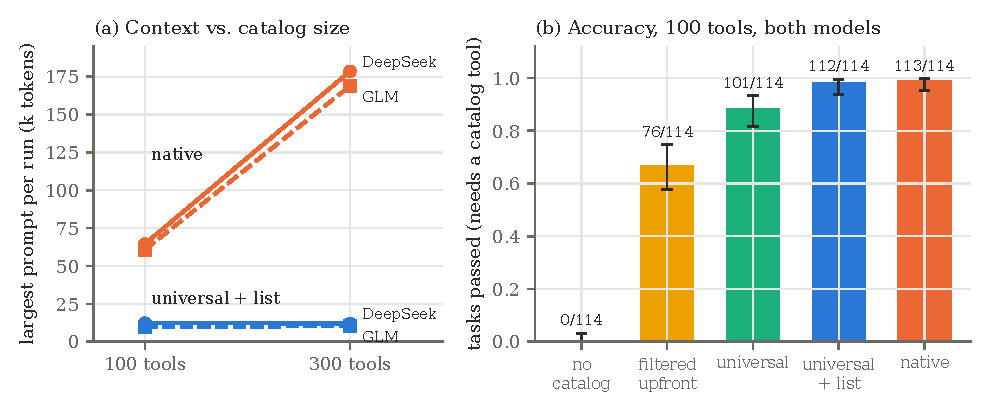
\includegraphics[width=0.85\textwidth]{../figures/fig_harness.pdf}
\caption{(a) The largest prompt of a run grows with the catalog when every definition is loaded and stays flat
with the universal tool (means over runs). (b) Share of runs passed on the 19 tasks that need a catalog tool
(single, mid-task, contract), 100 tools, both models pooled, with Wilson 95\% intervals.}
\label{fig:harness}
\end{figure*}

\textbf{The universal tool with a service list matches native.} On tasks that need a catalog tool it passed
112 of 114 runs, against 113 of 114 for native (Fig.~\ref{fig:harness}b); paired by task, model and repeat, one
run passed only with the universal tool and two only with native ($p=1$). It read 81\% less context per run
(Table~\ref{tab:main}): the largest prompt fell from 61--65k to 10--12k tokens and the context read over a whole
run from 324--461k to 60--88k, at about a quarter of native's cost, for about one extra step per run.

\textbf{Without the list, the universal tool loses some accuracy.} It passed 101 of 114 runs; against native
the paired difference is significant (0 vs.\ 12 discordant runs, $p=0.0005$), almost entirely through GLM.

\textbf{The tasks need the catalog, and the controls do not.} Without a catalog no run passed a task that needs
one (0 of 114); every control and absent task passed in every condition (Table~\ref{tab:cats}), and no control
run touched the catalog.

\begin{table}[t]
\caption{Pass Rate by Task Category, 100 Tools, Both Models}
\label{tab:cats}
\centering\footnotesize
\setlength{\tabcolsep}{4pt}
\begin{tabular}{@{}lccccc@{}}
\toprule
Category (tasks) & none & native & filtered & universal & + list \\
\midrule
control (6) & 1.00 & 1.00 & 1.00 & 1.00 & 1.00 \\
single (11) & 0.00 & 1.00 & 0.97 & 0.94 & 1.00 \\
mid-task (7) & 0.00 & 0.98 & \textbf{0.14} & 0.79 & 0.95 \\
contract (1) & 0.00 & 1.00 & 1.00 & 1.00 & 1.00 \\
absent (5) & 1.00 & 1.00 & 1.00 & 1.00 & 1.00 \\
\bottomrule
\end{tabular}
\end{table}

%=====================================================================
\section{Does It Hold as the Catalog Grows?}\label{sec:scale}
%=====================================================================
A larger catalog with near-duplicate services is harder for the DM. Table~\ref{tab:sweep} compares the 300-tool runs with the 100-tool runs of the same
repeats.

\begin{table}[t]
\caption{100 vs.\ 300 Catalog Tools (Repeats 0--1 at Both Sizes)}
\label{tab:sweep}
\centering\footnotesize
\setlength{\tabcolsep}{2.6pt}
\begin{tabular}{@{}llcccccc@{}}
\toprule
& & \multicolumn{2}{c}{Pass rate} & \multicolumn{2}{c}{Largest prompt} & \multicolumn{2}{c}{Context / run} \\
\cmidrule(lr){3-4}\cmidrule(lr){5-6}\cmidrule(l){7-8}
Model & Condition & 100 & 300 & 100 & 300 & 100 & 300 \\
\midrule
DeepSeek & native & 1.000 & 0.967 & 64.5k & 178.5k & 459k & 1,306k \\
 & universal & 0.983 & 1.000 & 11.2k & 12.0k & 80k & 90k \\
 & + list & 1.000 & 1.000 & 11.5k & 12.1k & 79k & 87k \\
GLM & native & 0.983 & 1.000 & 60.7k & 168.9k & 319k & 908k \\
 & universal & 0.867 & 0.883 & 9.3k & 9.0k & 64k & 62k \\
 & + list & 0.967 & 0.983 & 9.6k & 10.5k & 61k & 70k \\
\bottomrule
\end{tabular}
\end{table}

\textbf{Native's context nearly triples; the universal tool's barely moves.} With 300 tools the largest native
prompt reached 169--178k tokens and a run read 0.9--1.3 million; the universal tool with a service list stayed
at 10--12k and 70--87k, 92--93\% less context read per run (Fig.~\ref{fig:harness}a). Native's cost per run rose
from \$0.023--0.026 to \$0.064--0.071; the universal tool's from \$0.006 to \$0.008.

\textbf{Accuracy held.} On the tasks that need the catalog, the universal tool with a service list passed 75 of
76 runs at 300 tools and native 74 of 76. Native's two failures were DeepSeek runs that never found a mid-task
tool among 300 definitions and abstained; the universal tool's one failure was the GLM mid-task run that also
failed at 100 tools. No difference in this sweep is significant (universal + list vs.\ native: 2 vs.\ 1
discordant runs, $p=1$).

\textbf{The DM was not the bottleneck.} Its top three contained a needed tool for 86--95\% of
\texttt{find\_tool} calls at 300 tools (87--91\% at 100), despite the near-duplicate services; agents that missed
searched again. In earlier experiments outside the agent loop (in the artifact), \msd{} picked the right tool
among 200 BFCL tools for 94.7\% of items against 86.0\% for an LLM, at about a tenth of the cost.

%=====================================================================
\section{What Breaks the Universal Tool?}\label{sec:breaks}
%=====================================================================
\textbf{An agent does not search for what it does not know exists.} Of the 13 failures of the universal tool
without a service list (100 tools), 10 are runs in which the agent never called \texttt{find\_tool}: it did not
suspect that a tool for, say, the SLO target existed, and abstained. Eleven of the 13 are GLM runs. In no
failure did the DM fail to return a needed tool when asked. With the service list every run that needed the
catalog searched; its only two failures found the right tool for the first step of a two-step chain and did
not complete the second.

\textbf{Selecting tools upfront misses needs that appear mid-task.} The filtered condition chose five tools once,
from the task prompt. That suffices when the prompt names the need (0.97 on single lookups) and fails when a
need is revealed by the first lookup: on mid-task tasks the shortlist contained every needed tool in 14\% of
runs, and 36 of filtered's 38 failures trace to a missing tool.

\textbf{False positives were rare} (Table~\ref{tab:fp}). No condition invented a value: on the five absent tasks
every run abstained, and every value-task run that did not reach the right value abstained rather than
changing it. State-changing catalog calls occurred about once per 100 native and filtered runs, and one
universal run passed without calling the needed tool.

\begin{table}[t]
\caption{False Positives and Extra Activity per Run, 100 Tools (180 Runs per Condition; Lucky Passes Out of
114 Runs That Need the Catalog)}
\label{tab:fp}
\centering\footnotesize
\setlength{\tabcolsep}{3pt}
\begin{tabular}{@{}lcccccc@{}}
\toprule
 & Invented & State- & Unknown & Failed & Extra & Lucky \\
Condition & values & changing & tools & calls & calls & passes \\
\midrule
native & 0 & 0.01 & 0.00 & 0.55 & 2.03 & 0 \\
filtered & 0 & 0.01 & 0.00 & 2.35 & 2.21 & 0 \\
universal & 0 & 0.00 & 0.00 & 0.77 & 1.04 & 1 \\
universal + list & 0 & 0.00 & 0.02 & 0.67 & 1.82 & 0 \\
\bottomrule
\end{tabular}
\end{table}

\textbf{Blocked agents probe their environment.} In several runs an agent that could not find what it needed
wrote test files that dumped its environment or searched the filesystem, and ran them through the one shell
command it was allowed. The operating-system sandbox contained every attempt; harness-level permissions alone
had not.

%=====================================================================
\section{Can the Decision Model Make the Calls Itself?}\label{sec:calls}
%=====================================================================
Could the DM also choose the agent's next tool? We replayed
the 395 tool decisions of the session of Section~\ref{sec:overhead}: at each decision \msd{} and a second DM
(TypeSafe Jev~1.14~\cite{typesafejev}) saw the user's latest request and the agent's last eight steps, about
2,000 tokens against the agent's median of 340,000, and chose among the 38 tools the agent could call
(Table~\ref{tab:replay}). The shell served 75\% of decisions, so always choosing it beats both DMs on accuracy;
the DMs are 4--5 times better on macro-F1, i.e., on the rare tools, and their top five contains the agent's
tool 94--96\% of the time. On 300 steps of public OpenHands trajectories~\cite{wang2025openhands} on
SWE-rebench~\cite{badertdinov2025swerebench}, no system significantly beat ``always run bash''. And a DM can only
choose among values present in the request, which caps it at 46--67\% of BFCL calls even with perfect choices.
A coding agent's core tool choice is nearly trivial, and the hard part, writing commands and arguments, is
generation. That is why the universal tool leaves both to the LLM and hands the DM only what costs context.

\begin{table}[t]
\caption{Predicting a Real Coding Agent's Next Tool (395 Decisions, 38 Tools; Macro Scores Weight the 13 Used
Tools Equally)}
\label{tab:replay}
\centering\footnotesize
\setlength{\tabcolsep}{4pt}
\begin{tabular}{@{}lcccc@{}}
\toprule
Predictor & Accuracy & Macro recall & Macro F1 & Top-5 \\
\midrule
Always Bash & \textbf{0.754} & 0.077 & 0.066 & -- \\
Repeat previous tool & 0.597 & 0.108 & 0.108 & -- \\
\msd{} & 0.489 & 0.374 & \textbf{0.310} & 0.944 \\
Jev & 0.597 & 0.389 & 0.267 & 0.957 \\
\bottomrule
\end{tabular}
\end{table}

%=====================================================================
\section{Discussion}\label{sec:discussion}
%=====================================================================
Decision models do not replace the agent's own calls, but they can replace the part of tool calling that grows
with an organization: knowing every tool that exists. Selection is a choice among described options, which is
what a DM is trained for, and its cost does not grow with the catalog the way the prompt does: about
\$0.0001--0.0004 per search. We suggest:
(1)~keep the core coding tools native; (2)~put the catalog behind \texttt{find\_tool} and \texttt{call\_tool},
resolved at the moment of need; (3)~tell the agent, in one line per service, what the catalog covers; (4)~do
not preselect tools from the task text alone; (5)~run agents that reach internal services inside an
operating-system sandbox, not only behind harness permissions.

%=====================================================================
\section{Threats to Validity}\label{sec:threats}
%=====================================================================
\textbf{Internal.} Native passed about 99\% of runs, so these tasks can show that the universal tool loses no
accuracy, not that it gains any. Abstention was prompted: every value task offered an explicit way to abstain.
The 300-tool sweep has two repeats, so its comparisons have low power. Tokens and costs come from the agent's
own accounting, checked against the provider's bill (within 1\% for the 100-tool runs, 17\% for the last
300-tool batch).
\textbf{External.} The catalog and tasks are synthetic: descriptions are templated and more uniform than real
ones, and tasks are short (5--8 steps on average). We ran one agent, two inexpensive LLMs and one DM; frontier
models were not run for cost reasons. The session analysis covers one session of one agent.
\textbf{Construct.} Hidden tests check the needed value and behavior, not code quality; we additionally classify
every value-task outcome (correct, abstained, unchanged, wrong) and count false-positive signals.

%=====================================================================
\section{Conclusion}
%=====================================================================
Decision models can replace a coding agent's tool catalog. In a sandboxed coding-agent benchmark, a single
universal tool resolved by a decision model at the moment of need kept the agent's context flat as the catalog
grew from 100 to 300 tools, cutting it by 81--93\% with no detectable loss of accuracy, provided the agent is
told which services exist. They do not replace the agent's own tool calls, which need generation.

\section*{Data Availability}
The harness (catalog generator, MCP server, LLM proxy, sandbox setup, runner), the 30 tasks with hidden tests
and reference solutions, and the analysis scripts are available at \artifact.

\section*{Use of Generative AI}
Claude Code, Anthropic's coding agent, helped throughout this work: it wrote the harness, catalog, tasks and
analysis scripts, ran the experiments, and drafted the paper, under the authors' direction. The authors chose
the research questions, reviewed the code, results and text, and are responsible for the content. The session
analyzed in Sections~\ref{sec:overhead} and~\ref{sec:calls} is this assistant's own session.

\bibliographystyle{ieeetr}
\bibliography{../references}

\end{document}
"
\newcommand{\msd}{MSD1}
\newcommand{\artifact}{\ifanon\url{https://anonymous.4open.science/r/XXXX}\else\url{https://github.com/AzizMuminov/decision_models_for_tool_calling}\fi}
\let\oldus\_\renewcommand{\_}{\oldus\discretionary{}{}{}}

\begin{document}

\title{Can Decision Models Replace Tool Calling\\for Coding Agents?}

\ifanon
\author{\IEEEauthorblockN{Anonymous Author(s)}}
\else
\author{\IEEEauthorblockN{Aziz Muminov}
\and
\IEEEauthorblockN{Alexandra Ilyina}}
\fi

\maketitle

\begin{abstract}
Coding agents increasingly carry large tool catalogs, and every request re-sends every tool definition. We
test whether a decision model (DM), a model that returns a probability for each of a set of caller-supplied
options without generating text, can take the catalog's place. We built a sandboxed coding-agent benchmark:
an unmodified open-source agent works on 30 Python repositories whose hidden tests require facts available
only through a fictional company's internal catalog of 100 or 300 tools. Instead of the catalog, the agent
gets one universal tool: it states what it needs, a DM picks the matching tools, and the agent calls one.
Across 1,260 runs with two LLMs, the universal tool matched loading every definition (98--99\% vs.\
97--99\% success on tasks that need the catalog) while reading 81\% less context per run with 100 tools and
92--93\% less with 300. Two conditions matter: the agent must be told which services exist, and tools must
be selected when the need arises rather than upfront. The DM does not replace the agent's own calls; it
replaces the catalog.
\end{abstract}

\begin{IEEEkeywords}
coding agents, tool calling, decision models, Model Context Protocol
\end{IEEEkeywords}

%=====================================================================
\section{Introduction}\label{sec:intro}
%=====================================================================
A coding agent acts through tools: a shell, file reading and editing, search, and, increasingly, the tools of
every service its organization exposes through protocols such as MCP~\cite{mcp}: issue trackers, CI systems,
configuration services, documentation, databases. Each tool comes with a definition (a description and a
parameter schema) that the agent's LLM reads on every request, whether or not the tool is used. In the agent
session in which this paper's experiments were built, 51 always-loaded tool definitions took about 59,000
tokens, 93\% of the first request, and were re-sent with each of 435 requests; the agent used 10 of them
(Section~\ref{sec:overhead}). The coding agent we test documents the same problem: tool servers ``tend to add
a lot of tokens and can easily exceed the context limit''~\cite{opencode}.

\emph{Decision models} (DMs), released by several vendors in 2026~\cite{typesafejev,msd1,openrouterdecisions},
are built for choices. A DM reads a state and answers typed questions (yes/no, pick one of these options, give
a score) with a probability per option, in one forward pass, with no generated tokens, in well under a second
and for about \$0.04 per million input tokens. Finding the right tool in a catalog is such a choice. We
therefore replace the catalog with a \emph{universal tool} (Fig.~\ref{fig:universal}): the agent keeps its core
coding tools and gets two more, \texttt{find\_tool(intent)}, which a DM resolves against the full catalog at the
moment the agent asks, and \texttt{call\_tool(name, arguments)}. The catalog leaves the prompt; the LLM still
writes the intent, the arguments and the code.

\begin{figure}[t]
\centering
\resizebox{\columnwidth}{!}{%
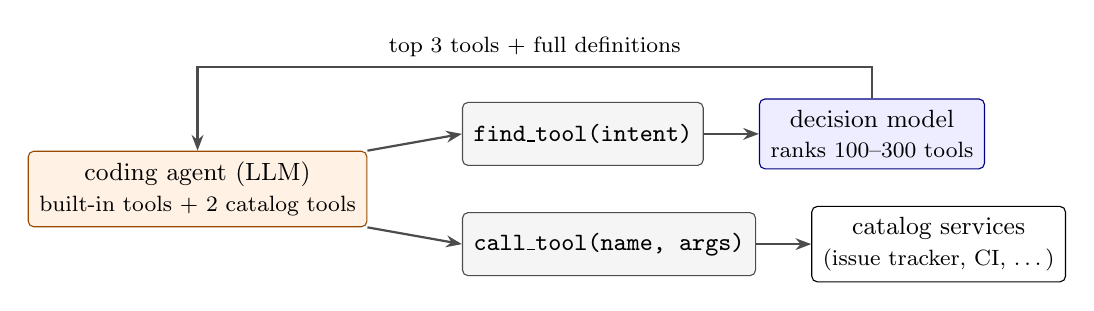
\begin{tikzpicture}[font=\small, node distance=5mm and 7mm,
  box/.style={draw, rounded corners=2pt, align=center, inner sep=4pt, minimum height=8mm, fill=white},
  dm/.style={box, fill=blue!7, draw=blue!50!black}, llm/.style={box, fill=orange!10, draw=orange!60!black},
  outb/.style={box, fill=gray!8, draw=gray!60!black}, arr/.style={-{Stealth[length=2mm]}, thick, draw=gray!60!black}]
\node[llm] (agent) {coding agent (LLM)\\ \footnotesize built-in tools + 2 catalog tools};
\node[outb, right=12mm of agent, yshift=7mm] (find) {\texttt{find\_tool(intent)}};
\node[dm, right=of find] (dm) {decision model\\ \footnotesize ranks 100--300 tools};
\node[outb, right=12mm of agent, yshift=-7mm] (call) {\texttt{call\_tool(name, args)}};
\node[box, right=of call] (svc) {catalog services\\ \footnotesize (issue tracker, CI, \dots)};
\draw[arr] (agent.north east) -- (find.west);
\draw[arr] (find) -- (dm);
\draw[arr] (dm.north) -- ++(0,4mm) -| node[pos=0.25, above, font=\footnotesize]{top 3 tools + full definitions} (agent.north);
\draw[arr] (agent.south east) -- (call.west);
\draw[arr] (call) -- (svc);
\end{tikzpicture}}
\caption{The universal tool. The agent's prompt holds two short tool definitions instead of the catalog; the
decision model resolves each stated intent at the moment the agent needs it.}
\label{fig:universal}
\end{figure}

Whether this works is a question about the whole agent loop, not about single calls: the agent must decide
to look for a capability it cannot see, describe it well enough, and use what comes back. We therefore built
a coding-agent benchmark for it (Section~\ref{sec:bench}). An unmodified open-source coding
agent~\cite{opencode} runs in an operating-system sandbox on 30 small Python repositories whose hidden tests
require values that only a fictional company's internal services return, through a catalog of 100 or 300
realistic tools; some needs appear only after a first lookup, and some values do not exist at all. We compare
five ways of exposing the catalog with two LLMs in 1,260 runs, and find:
\begin{itemize}
\item \textbf{The universal tool matches loading the whole catalog.} With a one-line list of the services, it
passed 112 of 114 runs that need the catalog against 113 for native tool calling at 100 tools, and 75 of 76
against 74 at 300 tools.
\item \textbf{It removes most of the context.} The largest prompt fell from 61--65k to 10--12k tokens at 100
tools and from 169--178k to 10--12k at 300; context read per run fell by 81\% and 92--93\%.
\item \textbf{Two design choices decide whether it works.} Without the service list, agents sometimes never
search for a capability they do not know exists; choosing tools once from the task prompt solved 14\% of
tasks whose needs appear mid-task.
\item \textbf{No condition invented a value}: where the value did not exist, every run abstained.
\end{itemize}
The DM's role is selection only: on the tool decisions of a real coding session it predicted the agent's next
tool less often than always choosing the shell (Section~\ref{sec:calls}).

\textbf{Contributions.} (i)~A sandboxed coding-agent benchmark for tool catalogs: an unmodified open-source
agent, a fictional 100/300-tool catalog, 30 tasks with hidden tests, five tool-exposure conditions, and
false-positive and abstention accounting. (ii)~Evidence from 1,260 runs that a DM-backed universal tool
preserves task success at a fraction of the context. (iii)~An analysis of its failure modes and a design
recipe. (iv)~A measurement of what tool definitions cost in a real coding session. Code, tasks and run
records are publicly available (see Data Availability).

%=====================================================================
\section{Background and Related Work}\label{sec:background}
%=====================================================================
\textbf{Decision models.} We use OpenRouter's Decisions API~\cite{openrouterdecisions}: a request carries a
\emph{state} and named questions of type yes/no, \texttt{choice} (one of named options, each with a free-text
description; returns a distribution) or \texttt{score}. We use Microsoft-Decision-1 (\msd{}), a post-trained
Qwen3.5-9B~\cite{msd1}; it rejects a \texttt{choice} with more than 255 options and requests beyond 32k
tokens. The Artificial Analysis Decision Index~\cite{aa2026decisionindex,olson2026decision} compares DMs with
LLMs on standalone tasks and finds them about even on tool-call routing; it does not place a DM inside an
agent.

\textbf{Too many tools.} Retrieving tools before generation is the standard answer to large
catalogs~\cite{qin2023toolllm,oats2026}; Lee~\cite{selection2026retrieval} finds that selecting a tool is
largely retrieval while recognizing that none applies is the hard part. Agent harnesses increasingly defer
tool definitions and load them on demand by keyword search. We test a learned, semantic version of this idea
inside an unmodified coding agent and measure its effect on end-to-end task success. Work on \emph{whether} to
call a tool at all~\cite{ross2025when2call,qian2025smart,tocall2026,sun2026probe} is complementary.

\textbf{Benchmarks.} Tool-calling benchmarks such as BFCL~\cite{patil2025bfcl} score single calls with small
menus; agentic benchmarks score task completion~\cite{yao2024taubench,mcpatlas2026,toolathlon2025}, and their
evaluators are themselves noisy~\cite{audit2026}. We therefore score tasks by hidden unit tests, in a fictional
organization whose tools no model can have seen.

%=====================================================================
\section{What Do Tool Definitions Cost?}\label{sec:overhead}
%=====================================================================
We parsed the full transcript of the coding session in which this paper's experiments were built (one agent,
32 user requests, 453 tool calls in 395 decisions, 435 LLM requests). Its 51 always-loaded tool definitions
took about 58,900 tokens (calibrated against the first request, 63,454 tokens before any conversation) and
were re-sent with every request: about 25 million of the 162 million context tokens the session read (16\%).
Two items alone cost about 39,000 tokens per request and were called once between them. Real definitions
averaged about 1,150 tokens (MCP tools: about 700), against about 150 in BFCL. Prompt caching makes these
tokens cheap but not free: at the session model's cached-read price (\$0.20 per million) they cost about \$5
of a \$60 session, and they occupy the context window on every request. Without caching, 100 tools of 700
tokens cost about \$280 per thousand requests at \$4 per million input tokens, against about \$0.50 per
thousand DM calls that each select among 200 tools.

%=====================================================================
\section{A Coding-Agent Benchmark for Tool Catalogs}\label{sec:bench}
%=====================================================================
\textbf{Harness.} We run opencode~\cite{opencode} (v1.19.4), an open-source coding agent, unmodified and
headless. It keeps its built-in tools (read, edit, glob, grep, list, a to-do list, and a shell restricted to
running \texttt{pytest}) in every condition; web access is off. The catalog is served by our MCP server over
local HTTP.

\textbf{Sandbox.} A first pilot with harness-level permissions only was invalid: the agent read the hidden
tests and answer files of its own task through absolute paths, and the no-catalog condition ``passed'' tasks
it could not solve. All reported runs therefore execute as an unprivileged operating-system user with an empty
environment, in a fresh copy of the task. The experiment's files and the API key are readable only by root;
the LLM is reached through a local proxy that adds the key and admits only the two experiment models. We
scanned every transcript for file access outside the task folder: 75 of 1,260 runs mentioned such a path, and
on inspection none read a protected file.

\textbf{Catalog.} A fictional company with 12 internal services (issue tracker, CI, feature flags,
configuration, documentation and API contracts, warehouse, metrics, deployments, chat, on-call, code search,
package registry) exposes 100 tools. Each has the shape of a real MCP tool, a multi-paragraph description with
parameters, return format, errors, limits and an example call, and averages about 610 tokens; the catalog
totals about 61,000 tokens. A 300-tool catalog adds 20 services, several deliberately close to an original one
(a support desk beside the issue tracker, A/B experiments beside feature flags), for about 184,000 tokens.
Every tool answers deterministically from a per-task world file: the right tool with sensible arguments returns
the needed fact, anything else an empty list or \texttt{NOT\_FOUND}.

\textbf{Tasks.} Thirty small Python repositories, each scored by hidden tests: \emph{control}~(6) bugs fixable
from the repository alone; \emph{single}~(11) the code must use one value that only a catalog tool returns (a
production configuration value, a feature flag, a package version, an SLO target, a CI threshold, \dots);
\emph{mid-task}~(7) the first lookup (a ticket, a chat thread, a docs page, a CI log) points to a second
service, so the second need cannot be predicted from the prompt; \emph{contract}~(1) implement a parser from
an API contract; and \emph{absent}~(5) the value does not exist anywhere the agent can reach. Every value
prompt ends with the same escape clause: if the authoritative value cannot be found, leave it unchanged and
add a \texttt{TODO: value not found} comment. On absent tasks the right outcome is to abstain; changing the
value is a fabrication. Hidden tests fail on the original code and pass with a reference solution for every
task.

\textbf{Conditions} (Table~\ref{tab:hconditions}). In the universal conditions, \texttt{find\_tool} asks \msd{}
to rank the catalog against the stated intent and returns the top three tools with their full definitions.
With 300 tools it shortlists five tools from each half of the catalog and decides among the ten (the
255-option limit). The service-list variant adds one line per service to \texttt{find\_tool}'s description,
about 170 tokens for 12 services and 430 for 32.

\begin{table}[t]
\caption{Tool-Exposure Conditions (Built-In Coding Tools Present in All)}
\label{tab:hconditions}
\centering\footnotesize
\begin{tabularx}{\columnwidth}{@{}l X@{}}
\toprule
Condition & What the agent sees of the catalog \\
\midrule
none & nothing (shows which tasks need the catalog) \\
native & every catalog tool with its full definition, in every request \\
filtered & the 5 tools \msd{} ranks highest for the task prompt, chosen once before the run \\
universal & \texttt{find\_tool} and \texttt{call\_tool}; no hint of what the catalog contains \\
universal + list & the same, plus a one-line list of the services the catalog covers \\
\bottomrule
\end{tabularx}
\end{table}

\textbf{Models and runs.} Two LLMs drive the agent: DeepSeek~V4.1~Flash and GLM-5.3, both with 1M-token context
windows. With 100 tools, each task ran under all five conditions with both models three times (900 runs); with
300 tools, native and both universal conditions ran twice (360 runs). We report pass rates with 95\%
confidence intervals that resample whole tasks, exact McNemar tests on runs paired by task, model and repeat,
and the tokens and cost opencode records per request (within 1\% of the provider's bill for the 900 runs).

%=====================================================================
\section{Can a Decision Model Replace the Tool Catalog?}\label{sec:catalog}
%=====================================================================
\begin{table*}[t]
\caption{Main Results, 100-Tool Catalog (30 Tasks $\times$ 3 Repeats per Row). Pass Rate Over All Tasks With a
Task-Clustered 95\% CI; Other Columns Are Means Over Runs.}
\label{tab:main}
\centering\footnotesize
\begin{tabular}{@{}llccrrr@{}}
\toprule
Model & Condition & Pass rate [95\% CI] & Steps & Largest prompt & Context read / run & Cost / run \\
\midrule
DeepSeek V4.1 Flash & none & 0.367 [0.20, 0.53] & 7.0 & 8,193 & 50,537 & \$0.0049 \\
 & native & 1.000 [1.00, 1.00] & 7.2 & 64,536 & 460,805 & \$0.0266 \\
 & filtered & 0.789 [0.63, 0.92] & 8.0 & 11,919 & 89,322 & \$0.0080 \\
 & universal & 0.978 [0.94, 1.00] & 8.4 & 11,269 & 81,047 & \$0.0066 \\
 & universal + list & \textbf{1.000} [1.00, 1.00] & 8.0 & 12,297 & 88,417 & \$0.0067 \\
\midrule
GLM-5.3 & none & 0.367 [0.20, 0.53] & 6.7 & 6,866 & 42,714 & \$0.0040 \\
 & native & 0.989 [0.97, 1.00] & 5.4 & 60,631 & 324,141 & \$0.0233 \\
 & filtered & 0.789 [0.63, 0.92] & 6.3 & 9,873 & 60,699 & \$0.0058 \\
 & universal & 0.878 [0.78, 0.97] & 7.5 & 9,139 & 61,954 & \$0.0059 \\
 & universal + list & \textbf{0.978} [0.93, 1.00] & 6.6 & 9,593 & 60,028 & \$0.0055 \\
\bottomrule
\end{tabular}
\end{table*}

\begin{figure*}[t]
\centering
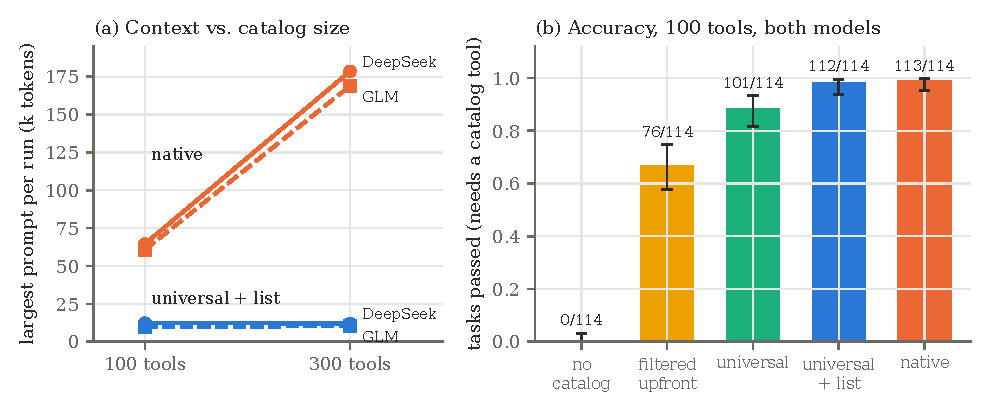
\includegraphics[width=0.85\textwidth]{../figures/fig_harness.pdf}
\caption{(a) The largest prompt of a run grows with the catalog when every definition is loaded and stays flat
with the universal tool (means over runs). (b) Share of runs passed on the 19 tasks that need a catalog tool
(single, mid-task, contract), 100 tools, both models pooled, with Wilson 95\% intervals.}
\label{fig:harness}
\end{figure*}

\textbf{The universal tool with a service list matches native.} On tasks that need a catalog tool it passed
112 of 114 runs, against 113 of 114 for native (Fig.~\ref{fig:harness}b); paired by task, model and repeat, one
run passed only with the universal tool and two only with native ($p=1$). It read 81\% less context per run
(Table~\ref{tab:main}): the largest prompt fell from 61--65k to 10--12k tokens and the context read over a whole
run from 324--461k to 60--88k, at about a quarter of native's cost, for about one extra step per run.

\textbf{Without the list, the universal tool loses some accuracy.} It passed 101 of 114 runs; against native
the paired difference is significant (0 vs.\ 12 discordant runs, $p=0.0005$), almost entirely through GLM.

\textbf{The tasks need the catalog, and the controls do not.} Without a catalog no run passed a task that needs
one (0 of 114); every control and absent task passed in every condition (Table~\ref{tab:cats}), and no control
run touched the catalog.

\begin{table}[t]
\caption{Pass Rate by Task Category, 100 Tools, Both Models}
\label{tab:cats}
\centering\footnotesize
\setlength{\tabcolsep}{4pt}
\begin{tabular}{@{}lccccc@{}}
\toprule
Category (tasks) & none & native & filtered & universal & + list \\
\midrule
control (6) & 1.00 & 1.00 & 1.00 & 1.00 & 1.00 \\
single (11) & 0.00 & 1.00 & 0.97 & 0.94 & 1.00 \\
mid-task (7) & 0.00 & 0.98 & \textbf{0.14} & 0.79 & 0.95 \\
contract (1) & 0.00 & 1.00 & 1.00 & 1.00 & 1.00 \\
absent (5) & 1.00 & 1.00 & 1.00 & 1.00 & 1.00 \\
\bottomrule
\end{tabular}
\end{table}

%=====================================================================
\section{Does It Hold as the Catalog Grows?}\label{sec:scale}
%=====================================================================
A larger catalog with near-duplicate services is harder for the DM. Table~\ref{tab:sweep} compares the 300-tool runs with the 100-tool runs of the same
repeats.

\begin{table}[t]
\caption{100 vs.\ 300 Catalog Tools (Repeats 0--1 at Both Sizes)}
\label{tab:sweep}
\centering\footnotesize
\setlength{\tabcolsep}{2.6pt}
\begin{tabular}{@{}llcccccc@{}}
\toprule
& & \multicolumn{2}{c}{Pass rate} & \multicolumn{2}{c}{Largest prompt} & \multicolumn{2}{c}{Context / run} \\
\cmidrule(lr){3-4}\cmidrule(lr){5-6}\cmidrule(l){7-8}
Model & Condition & 100 & 300 & 100 & 300 & 100 & 300 \\
\midrule
DeepSeek & native & 1.000 & 0.967 & 64.5k & 178.5k & 459k & 1,306k \\
 & universal & 0.983 & 1.000 & 11.2k & 12.0k & 80k & 90k \\
 & + list & 1.000 & 1.000 & 11.5k & 12.1k & 79k & 87k \\
GLM & native & 0.983 & 1.000 & 60.7k & 168.9k & 319k & 908k \\
 & universal & 0.867 & 0.883 & 9.3k & 9.0k & 64k & 62k \\
 & + list & 0.967 & 0.983 & 9.6k & 10.5k & 61k & 70k \\
\bottomrule
\end{tabular}
\end{table}

\textbf{Native's context nearly triples; the universal tool's barely moves.} With 300 tools the largest native
prompt reached 169--178k tokens and a run read 0.9--1.3 million; the universal tool with a service list stayed
at 10--12k and 70--87k, 92--93\% less context read per run (Fig.~\ref{fig:harness}a). Native's cost per run rose
from \$0.023--0.026 to \$0.064--0.071; the universal tool's from \$0.006 to \$0.008.

\textbf{Accuracy held.} On the tasks that need the catalog, the universal tool with a service list passed 75 of
76 runs at 300 tools and native 74 of 76. Native's two failures were DeepSeek runs that never found a mid-task
tool among 300 definitions and abstained; the universal tool's one failure was the GLM mid-task run that also
failed at 100 tools. No difference in this sweep is significant (universal + list vs.\ native: 2 vs.\ 1
discordant runs, $p=1$).

\textbf{The DM was not the bottleneck.} Its top three contained a needed tool for 86--95\% of
\texttt{find\_tool} calls at 300 tools (87--91\% at 100), despite the near-duplicate services; agents that missed
searched again. In earlier experiments outside the agent loop (in the artifact), \msd{} picked the right tool
among 200 BFCL tools for 94.7\% of items against 86.0\% for an LLM, at about a tenth of the cost.

%=====================================================================
\section{What Breaks the Universal Tool?}\label{sec:breaks}
%=====================================================================
\textbf{An agent does not search for what it does not know exists.} Of the 13 failures of the universal tool
without a service list (100 tools), 10 are runs in which the agent never called \texttt{find\_tool}: it did not
suspect that a tool for, say, the SLO target existed, and abstained. Eleven of the 13 are GLM runs. In no
failure did the DM fail to return a needed tool when asked. With the service list every run that needed the
catalog searched; its only two failures found the right tool for the first step of a two-step chain and did
not complete the second.

\textbf{Selecting tools upfront misses needs that appear mid-task.} The filtered condition chose five tools once,
from the task prompt. That suffices when the prompt names the need (0.97 on single lookups) and fails when a
need is revealed by the first lookup: on mid-task tasks the shortlist contained every needed tool in 14\% of
runs, and 36 of filtered's 38 failures trace to a missing tool.

\textbf{False positives were rare} (Table~\ref{tab:fp}). No condition invented a value: on the five absent tasks
every run abstained, and every value-task run that did not reach the right value abstained rather than
changing it. State-changing catalog calls occurred about once per 100 native and filtered runs, and one
universal run passed without calling the needed tool.

\begin{table}[t]
\caption{False Positives and Extra Activity per Run, 100 Tools (180 Runs per Condition; Lucky Passes Out of
114 Runs That Need the Catalog)}
\label{tab:fp}
\centering\footnotesize
\setlength{\tabcolsep}{3pt}
\begin{tabular}{@{}lcccccc@{}}
\toprule
 & Invented & State- & Unknown & Failed & Extra & Lucky \\
Condition & values & changing & tools & calls & calls & passes \\
\midrule
native & 0 & 0.01 & 0.00 & 0.55 & 2.03 & 0 \\
filtered & 0 & 0.01 & 0.00 & 2.35 & 2.21 & 0 \\
universal & 0 & 0.00 & 0.00 & 0.77 & 1.04 & 1 \\
universal + list & 0 & 0.00 & 0.02 & 0.67 & 1.82 & 0 \\
\bottomrule
\end{tabular}
\end{table}

\textbf{Blocked agents probe their environment.} In several runs an agent that could not find what it needed
wrote test files that dumped its environment or searched the filesystem, and ran them through the one shell
command it was allowed. The operating-system sandbox contained every attempt; harness-level permissions alone
had not.

%=====================================================================
\section{Can the Decision Model Make the Calls Itself?}\label{sec:calls}
%=====================================================================
Could the DM also choose the agent's next tool? We replayed
the 395 tool decisions of the session of Section~\ref{sec:overhead}: at each decision \msd{} and a second DM
(TypeSafe Jev~1.14~\cite{typesafejev}) saw the user's latest request and the agent's last eight steps, about
2,000 tokens against the agent's median of 340,000, and chose among the 38 tools the agent could call
(Table~\ref{tab:replay}). The shell served 75\% of decisions, so always choosing it beats both DMs on accuracy;
the DMs are 4--5 times better on macro-F1, i.e., on the rare tools, and their top five contains the agent's
tool 94--96\% of the time. On 300 steps of public OpenHands trajectories~\cite{wang2025openhands} on
SWE-rebench~\cite{badertdinov2025swerebench}, no system significantly beat ``always run bash''. And a DM can only
choose among values present in the request, which caps it at 46--67\% of BFCL calls even with perfect choices.
A coding agent's core tool choice is nearly trivial, and the hard part, writing commands and arguments, is
generation. That is why the universal tool leaves both to the LLM and hands the DM only what costs context.

\begin{table}[t]
\caption{Predicting a Real Coding Agent's Next Tool (395 Decisions, 38 Tools; Macro Scores Weight the 13 Used
Tools Equally)}
\label{tab:replay}
\centering\footnotesize
\setlength{\tabcolsep}{4pt}
\begin{tabular}{@{}lcccc@{}}
\toprule
Predictor & Accuracy & Macro recall & Macro F1 & Top-5 \\
\midrule
Always Bash & \textbf{0.754} & 0.077 & 0.066 & -- \\
Repeat previous tool & 0.597 & 0.108 & 0.108 & -- \\
\msd{} & 0.489 & 0.374 & \textbf{0.310} & 0.944 \\
Jev & 0.597 & 0.389 & 0.267 & 0.957 \\
\bottomrule
\end{tabular}
\end{table}

%=====================================================================
\section{Discussion}\label{sec:discussion}
%=====================================================================
Decision models do not replace the agent's own calls, but they can replace the part of tool calling that grows
with an organization: knowing every tool that exists. Selection is a choice among described options, which is
what a DM is trained for, and its cost does not grow with the catalog the way the prompt does: about
\$0.0001--0.0004 per search. We suggest:
(1)~keep the core coding tools native; (2)~put the catalog behind \texttt{find\_tool} and \texttt{call\_tool},
resolved at the moment of need; (3)~tell the agent, in one line per service, what the catalog covers; (4)~do
not preselect tools from the task text alone; (5)~run agents that reach internal services inside an
operating-system sandbox, not only behind harness permissions.

%=====================================================================
\section{Threats to Validity}\label{sec:threats}
%=====================================================================
\textbf{Internal.} Native passed about 99\% of runs, so these tasks can show that the universal tool loses no
accuracy, not that it gains any. Abstention was prompted: every value task offered an explicit way to abstain.
The 300-tool sweep has two repeats, so its comparisons have low power. Tokens and costs come from the agent's
own accounting, checked against the provider's bill (within 1\% for the 100-tool runs, 17\% for the last
300-tool batch).
\textbf{External.} The catalog and tasks are synthetic: descriptions are templated and more uniform than real
ones, and tasks are short (5--8 steps on average). We ran one agent, two inexpensive LLMs and one DM; frontier
models were not run for cost reasons. The session analysis covers one session of one agent.
\textbf{Construct.} Hidden tests check the needed value and behavior, not code quality; we additionally classify
every value-task outcome (correct, abstained, unchanged, wrong) and count false-positive signals.

%=====================================================================
\section{Conclusion}
%=====================================================================
Decision models can replace a coding agent's tool catalog. In a sandboxed coding-agent benchmark, a single
universal tool resolved by a decision model at the moment of need kept the agent's context flat as the catalog
grew from 100 to 300 tools, cutting it by 81--93\% with no detectable loss of accuracy, provided the agent is
told which services exist. They do not replace the agent's own tool calls, which need generation.

\section*{Data Availability}
The harness (catalog generator, MCP server, LLM proxy, sandbox setup, runner), the 30 tasks with hidden tests
and reference solutions, and the analysis scripts are available at \artifact.

\section*{Use of Generative AI}
Claude Code, Anthropic's coding agent, helped throughout this work: it wrote the harness, catalog, tasks and
analysis scripts, ran the experiments, and drafted the paper, under the authors' direction. The authors chose
the research questions, reviewed the code, results and text, and are responsible for the content. The session
analyzed in Sections~\ref{sec:overhead} and~\ref{sec:calls} is this assistant's own session.

\bibliographystyle{ieeetr}
\bibliography{../references}

\end{document}
